% =================================================================
%  VAE presentation — FULL DECK (Part 1 + Part 2 + Part 3)
%  Each part is copied unchanged from its own file and kept inside a
%  \begingroup ... \endgroup, so its preamble (colours, TikZ styles,
%  macros, Beamer templates) cannot leak into the other parts.
%  Assets: assets/part1, assets/part2, assets/part3
%  Build: pdflatex twice.  The latent-walk animation plays in Adobe Acrobat/Reader.
% =================================================================
\documentclass[aspectratio=169,11pt]{beamer}

\usepackage{plex-serif}
\renewcommand{\familydefault}{\rmdefault}
\usepackage[T1]{fontenc}
\usepackage{amsmath,amssymb,bm}
\usepackage{pifont}
\usepackage{tikz}
\usepackage{etoolbox}
\usepackage{animate}
\usetikzlibrary{calc,positioning,shapes.geometric,shapes.symbols,arrows.meta,
                decorations.pathreplacing,overlay-beamer-styles}

\title{Variational Autoencoder}

% Beamer applies the normal-text colour once, at \begin{document}, so it
% has to be set here (all three parts use the same ink colour).
\definecolor{ink}{HTML}{1C2233}
\setbeamercolor{normal text}{fg=ink}

\begin{document}

% #################################################################
%  PART 1  (from part1/part1_final.tex, unchanged)
%  Wrapped in a group: its colours, styles, macros and templates
%  apply only to its own slides.
% #################################################################
\begingroup
\graphicspath{{assets/part1/}}
\renewcommand{\familydefault}{\rmdefault}

% ---------- Palette ----------
\definecolor{navy}{HTML}{002B55}
\definecolor{steel}{HTML}{4D6FAD}
\definecolor{sky}{HTML}{5DADF5}
\definecolor{teal}{HTML}{3F8C8A}
\definecolor{slate}{HTML}{5B6475}
\definecolor{paper}{HTML}{FBFAF7}
\definecolor{ink}{HTML}{1C2233}
\colorlet{deepteal}{navy!55!teal}
\definecolor{amber}{HTML}{E0A526}

% ---------- TikZ overlay helpers ----------
\tikzset{
  invisible/.style={opacity=0,text opacity=0},
  visible on/.style={alt={#1{}{invisible}}},
  alt/.code args={<#1>#2#3}{\alt<#1>{\pgfkeysalso{#2}}{\pgfkeysalso{#3}}},
  focus on/.style={alt={#1{draw=teal,line width=1.3pt}{}}},
  emphasis on/.style={alt={#1{draw=deepteal,line width=1.3pt,fill=deepteal!4}{}}},
}

% ---------- Standard diagram styles ----------
\tikzset{
  >={Stealth[length=2mm]},
  arr/.style={->,line width=0.7pt,draw=slate},
  lbl/.style={font=\footnotesize,text=slate,align=center},
  block/.style={trapezium,trapezium stretches=true,minimum width=2.4cm,minimum height=1.55cm,
                line width=0.8pt,font=\bfseries},
  enc/.style={block,shape border rotate=270,fill=steel!12,draw=steel,text=navy},
  dec/.style={block,shape border rotate=90,fill=teal!10,draw=teal,text=teal!70!black},
  param/.style={rectangle,rounded corners=2pt,minimum width=0.95cm,minimum height=0.6cm,
                draw=steel,line width=0.8pt,fill=white,text=navy,font=\normalsize},
  op/.style={circle,draw=slate,line width=0.8pt,fill=white,inner sep=1pt},
  photo/.style={draw=slate!50,line width=0.5pt},
  chip/.style={rectangle,rounded corners=3pt,line width=0.8pt,inner xsep=7pt,inner ysep=4pt,
               font=\footnotesize,fill=white},
  neuron/.style={circle,minimum size=0.48cm,inner sep=0pt,line width=0.7pt,font=\scriptsize},
  mystery/.style={rectangle,rounded corners=5pt,draw=deepteal,line width=1.3pt,fill=white,text=deepteal,
                  font=\fontsize{24}{24}\fontseries{eb}\selectfont},
}

% ---------- Beamer theme ----------
\setbeamercolor{background canvas}{bg=paper}
\setbeamercolor{normal text}{fg=ink}
\setbeamercolor{alerted text}{fg=teal}
\setbeamercolor{structure}{fg=navy}
\setbeamercolor{block title}{bg=navy,fg=white}
\setbeamercolor{block body}{bg=slate!7,fg=ink}
\setbeamertemplate{navigation symbols}{}
\setbeamertemplate{blocks}[rounded][shadow=false]

\newcommand{\stripeTR}[3]{\fill[#3] (#1,9.2) -- ++(#2,0) -- ++(4.5,-3.15) -- ++(-#2,0) -- cycle;}
\newcommand{\stripeBL}[3]{\fill[#3] (#1,-0.2) -- ++(#2,0) -- ++(-4.5,3.15) -- ++(-#2,0) -- cycle;}

\setbeamertemplate{background}{%
  \begin{tikzpicture}[remember picture,overlay,shift={(current page.south west)}]
    \clip (0,0) rectangle (16,9);
  \end{tikzpicture}}

\setbeamertemplate{frametitle}{%
  \begin{tikzpicture}[remember picture,overlay,shift={(current page.north west)}]
    \fill[navy] (0,0) rectangle (16,-1.05);
    \node[anchor=west,text=white,font=\fontseries{eb}\selectfont\Large] at (0.72,-0.525)
      {\insertframetitle};
  \end{tikzpicture}
  \vspace*{0.78cm}}


 \setbeamertemplate{footline}{%
  \begin{tikzpicture}[remember picture,overlay,shift={(current page.south west)}]
    \node[anchor=west,font=\scriptsize,text=steel] at (0.72,0.32)
      {Variational Autoencoder \;\textcolor{slate!60}{|}\; CSE 200};
    \node[anchor=east,font=\scriptsize\bfseries,text=steel] at (15.3,0.32)
      {\insertframenumber/\inserttotalframenumber};
  \end{tikzpicture}}


 \setbeamertemplate{footline}{%
  \begin{tikzpicture}[remember picture,overlay,shift={(current page.south west)}]
    \node[anchor=west,font=\scriptsize,text=steel] at (0.72,0.32)
      {Variational Autoencoder \;\textcolor{slate!60}{|}\; CSE200};
    \node[anchor=east,font=\scriptsize\bfseries,text=steel] at (15.3,0.32)
      {\insertframenumber/\inserttotalframenumber};
  \end{tikzpicture}}

% ---------- Page canvas: draw in page coordinates (16 x 9 cm) ----------
% content zone ~ x 0.9..15.1, y 0.9..7.3
\newenvironment{canvas}
  {\begin{tikzpicture}[remember picture,overlay,shift={(current page.south west)}]}
  {\end{tikzpicture}}

% ---------- Reusable drawings ----------
% digit "image" thumbnail:  \thumb[opts]{pos}{digit}
\newcommand{\thumb}[3][]{%
  \node[draw=slate!50,line width=0.5pt,fill=white,minimum size=0.52cm,inner sep=0pt,text=ink,
        font=\small\fontseries{eb}\selectfont,#1] at (#2) {#3};}

% latent-space clusters. #1 = cloud radius (0 = plain points), #2 = scale of cluster centres
\newcommand{\clusters}[2]{%
  \pgfmathsetseed{4242}%
  \foreach \cx/\cy/\sx/\sy/\rot/\col in {
      -2.35/ 1.55/0.34/0.20/ 20/navy,
      -0.25/ 1.85/0.20/0.40/-25/teal,
       2.20/ 1.20/0.40/0.22/ 40/steel,
      -2.05/-1.35/0.30/0.28/  0/slate,
       0.60/-0.45/0.26/0.36/ 60/teal!55!white,
       2.40/-1.65/0.44/0.19/-15/steel!55!white}{%
    \foreach \k in {1,...,22}{%
      \pgfmathsetmacro\rr{min(2.1,sqrt(-2*ln(max(rnd,0.005))))}%
      \pgfmathsetmacro\tt{360*rnd}%
      \pgfmathsetmacro\px{#2*\cx + cos(\rot)*\sx*\rr*cos(\tt) - sin(\rot)*\sy*\rr*sin(\tt)}%
      \pgfmathsetmacro\py{#2*\cy + sin(\rot)*\sx*\rr*cos(\tt) + cos(\rot)*\sy*\rr*sin(\tt)}%
      \ifdim #1pt>0pt \fill[\col,opacity={0.024/#1}] (\px,\py) circle (#1); \fi
      \fill[\col] (\px,\py) circle (0.055);
    }}}
% digit labels next to the clusters (#1 = centre scale)
\newcommand{\clusterlabels}[1]{%
  \foreach \cx/\cy/\dx/\dy/\d in {-2.35/1.55/-0.95/0.25/0, -0.25/1.85/0.55/0.3/1, 2.20/1.20/0.2/0.8/7,
                                  -2.05/-1.35/0.9/-0.5/3, 0.60/-0.45/-0.8/-0.5/5, 2.40/-1.65/-0.15/-0.75/9}
    {\thumb[minimum size=0.42cm,font=\scriptsize\fontseries{eb}\selectfont]{#1*\cx+\dx,#1*\cy+\dy}{\d}}}
% empty latent panel, centred at the current origin (7.4 x 5.9 cm)
\newcommand{\latentpanel}{%
  \fill[white] (-3.7,-2.95) rectangle (3.7,2.95);
  \begin{scope}
    \clip (-3.7,-2.95) rectangle (3.7,2.95);
    \draw[slate!12,line width=0.4pt,step=0.5] (-4,-3) grid (4,3);
    \draw[slate!30,line width=0.5pt] (-3.7,0) -- (3.7,0) (0,-2.95) -- (0,2.95);
  \end{scope}
  \draw[slate!50,line width=0.5pt] (-3.7,-2.95) rectangle (3.7,2.95);
  \node[lbl,anchor=north east] at (3.7,-2.95) {$z_1$};
  \node[lbl,anchor=north east] at (-3.7,2.95) {$z_2$};
  \node[anchor=north west,font=\scriptsize,text=slate] at (-3.62,2.9) {bottleneck (latent) space};}

% number line on [-1,1]:  \numline{pos}{width}
\newcommand{\numline}[2]{%
  \draw[slate!70,line width=0.5pt,<->,>={Stealth[length=1.2mm]}] ($(#1)+(-#2/2-0.18,0)$) -- ($(#1)+(#2/2+0.18,0)$);
  \foreach \v in {-1,0,1}
    \draw[slate!70,line width=0.5pt] ($(#1)+(\v*#2/2,0.05)$) -- ++(0,-0.1)
       node[below=-1.5pt,font=\tiny,text=slate] {$\v$};}
% gaussian on that number line:  \gauss{pos}{width}{mu}{sigma}{height}
\newcommand{\gauss}[5]{%
  \begin{scope}[shift={(#1)}]
    \fill[navy!10] plot[domain={max(-1,#3-3*#4)}:{min(1,#3+3*#4)},samples=45]
          ({\x*#2/2},{#5*exp(-((\x-(#3))^2)/(2*#4*#4))}) -- cycle;
    \draw[navy,line width=0.8pt] plot[domain={max(-1,#3-3*#4)}:{min(1,#3+3*#4)},samples=45]
          ({\x*#2/2},{#5*exp(-((\x-(#3))^2)/(2*#4*#4))});
  \end{scope}}

% face "photo":  \face{pos}{scale}{smile -1..1}{skin}{hair}{style 0 short|1 long|2 curly|3 beard}{bg}{shirt}
\newcommand{\face}[8]{%
  \begin{scope}[shift={(#1)},scale=#2]
    \fill[#7] (-0.6,-0.6) rectangle (0.6,0.6);
    \begin{scope}
      \clip (-0.6,-0.6) rectangle (0.6,0.6);
      \ifcase#6\relax
      \or \fill[#5] (-0.38,-0.62) -- (-0.4,0.06) arc (180:0:0.4) -- (0.38,-0.62) -- cycle;
      \or \foreach \a in {0,30,...,330} \fill[#5] ($(0,0.08)+(\a:0.3)$) circle (0.15);
      \fi
      \fill[#8] (-0.56,-0.62) .. controls (-0.52,-0.42) and (-0.32,-0.36) .. (0,-0.36)
                .. controls (0.32,-0.36) and (0.52,-0.42) .. (0.56,-0.62) -- cycle;
      \fill[#4!85!ink] (-0.09,-0.42) rectangle (0.09,-0.2);
      \fill[#4] (0,0.02) ellipse (0.26 and 0.32);
      \ifnum#6=1\relax\else
        \fill[#5] (-0.27,0.06) .. controls (-0.3,0.44) and (0.3,0.44) .. (0.27,0.06)
                  .. controls (0.18,0.22) and (-0.12,0.26) .. (-0.27,0.06) -- cycle;
      \fi
      \ifnum#6=1\relax
        \fill[#5] (-0.26,0.08) .. controls (-0.22,0.4) and (0.24,0.4) .. (0.26,0.08)
                  .. controls (0.1,0.26) and (-0.1,0.26) .. (-0.26,0.08) -- cycle;
      \fi
      \ifnum#6=3\relax
        \fill[#5] (-0.26,0.0) .. controls (-0.25,-0.42) and (0.25,-0.42) .. (0.26,0.0)
                  -- (0.19,-0.02) .. controls (0.14,-0.2) and (-0.14,-0.2) .. (-0.19,-0.02) -- cycle;
      \fi
      \fill[ink] (-0.1,0.07) circle (0.028) (0.1,0.07) circle (0.028);
      \draw[ink!70,line width=0.5pt] (-0.15,0.15) -- (-0.05,0.16) (0.05,0.16) -- (0.15,0.15);
      \ifnum#6=3\relax\def\mouthcol{white}\else\def\mouthcol{ink}\fi
      \draw[\mouthcol,line width=0.8pt,line cap=round]
            (-0.1,-0.13) .. controls (-0.04,{-0.13-0.11*(#3)}) and (0.04,{-0.13-0.11*(#3)}) .. (0.1,-0.13);
    \end{scope}
    \draw[slate!50,line width=0.5pt] (-0.6,-0.6) rectangle (0.6,0.6);
  \end{scope}}
% the recurring bearded person used on the VAE slides
\newcommand{\person}[2]{\face{#1}{#2}{0.75}{teal!55!white}{slate!55!ink}{3}{steel!10}{steel!60}}
% base phone mockup (no alert, no dimming)
\newcommand{\phonemockup}{%
  \fill[ink,rounded corners=10pt] (1.45,1.05) rectangle (4.65,7.25);
  \fill[white,rounded corners=7pt] (1.58,1.2) rectangle (4.52,7.1);
  \begin{scope}
    \clip[rounded corners=7pt] (1.58,1.2) rectangle (4.52,7.1);
    \node[anchor=north west,inner sep=0pt] at (1.58,6.36) {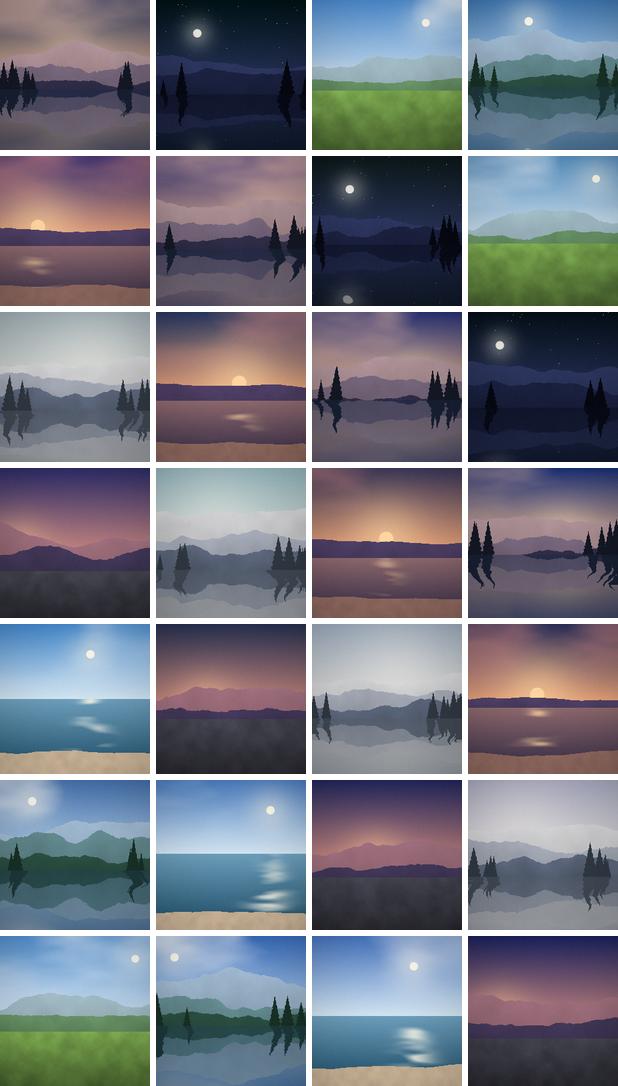
\includegraphics[width=2.94cm]{gallery.png}};
    \fill[white] (1.58,6.36) rectangle (4.52,7.1);
    \fill[white,opacity=0.92] (1.58,1.2) rectangle (4.52,1.55);
  \end{scope}
  \fill[ink,rounded corners=2pt] (2.8,6.93) rectangle (3.3,7.02);
  \node[anchor=west,font=\tiny\bfseries,text=ink] at (1.68,6.97) {9:41};
  \draw[ink,line width=0.4pt] (4.05,6.92) rectangle (4.33,7.02);
  \fill[teal] (4.07,6.94) rectangle (4.1,7.0);
  \node[anchor=west,font=\scriptsize\bfseries,text=ink] at (1.66,6.6) {Photos};
  \node[anchor=east,font=\tiny,text=slate] at (4.46,6.6) {20,000 items};
  \fill[slate!60,rounded corners=1pt] (2.6,1.3) rectangle (3.5,1.36);
}
% dims the screen (for the alert state)
\newcommand{\phonedim}{%
  \begin{scope}
    \clip[rounded corners=7pt] (1.58,1.2) rectangle (4.52,7.1);
    \fill[ink,opacity=0.45] (1.58,1.2) rectangle (4.52,7.1);
  \end{scope}}
% the storage-full popup
\newcommand{\storagealert}{%
  \fill[white,rounded corners=5pt] (1.78,3.15) rectangle (4.32,5.35);
  \draw[teal,line width=0.8pt,rounded corners=5pt] (1.78,3.15) rectangle (4.32,5.35);
  \fill[teal] (3.05,5.0) -- ++(-0.2,-0.35) -- ++(0.4,0) -- cycle;
  \node[font=\tiny\bfseries,text=white] at (3.05,4.77) {!};
  \node[font=\scriptsize\bfseries,text=ink] at (3.05,4.38) {Storage Almost Full};
  \node[font=\tiny,text=slate,align=center] at (3.05,4.0) {127.6 GB of 128 GB used};
  \fill[slate!15,rounded corners=1pt] (2.05,3.62) rectangle (4.05,3.72);
  \fill[teal,rounded corners=1pt] (2.05,3.62) rectangle (4.0,3.72);
  \node[font=\tiny\bfseries,text=steel] at (3.05,3.35) {Manage Storage};}

\newcommand{\cmark}{\ding{51}}
\newcommand{\xmark}{\ding{55}}

\title{Variational Autoencoder}
% slides: no hyphenation, ragged text
\hyphenpenalty=10000 \exhyphenpenalty=10000

% =================================================================
%  TITLE SLIDE  (deck opener — Part 1 starts the presentation)
% =================================================================

\begin{frame}[plain]
\begin{tikzpicture}[remember picture,overlay,shift={(current page.south west)}]
  \clip (0,0) rectangle (16,9);

  % ---------- slight background tint ----------
  \fill[steel!7] (0,0) rectangle (16,9);

  % ---------- text (centred) ----------
  \node[font=\small\bfseries,text=teal] at (8,7.1) {CSE200 \;\textbullet\; B2 \;\textbullet\; Group 2};
  \node[text=navy,align=center,font=\fontsize{32}{35}\fontseries{eb}\selectfont]
       at (8,5.5) {VARIATIONAL\\AUTOENCODER};
  \node[text=slate,font=\small] at (8,3.3) {Presented by};
  \node[text=ink,font=\small\bfseries] at (8,2.8)
       {Mahir Mahtab \;\textbullet\; Nusaiba Nehleen Bhuiyan \;\textbullet\; Ramisa Musarrat Sujana};
  \node[text=slate,font=\footnotesize\itshape] at (8,2.05) {Department of CSE, BUET};
\end{tikzpicture}
\end{frame}

% =================================================================
%  PAGE 1 — The problem: storage full
% =================================================================
% ---- Slide 1: phone + count ----
\begin{frame}{The Problem: Storage Almost Full}
\begin{canvas}
  \begin{scope}[shift={(2.45,0)}] \phonemockup \end{scope}
\node[anchor=base west,text=navy,font=\fontsize{44}{44}\fontseries{eb}\selectfont] (num) at (7.5,3.5) {20{,}000};
  \node[anchor=base west,text=steel,font=\Large] at ($(num.base east)+(0.11,0.3)$) {photos};
    \node[anchor=north west,text width=8.6cm,align=left,font=\normalsize,text=ink] at (7.5,5.6)
       {Imagine your phone has};
\end{canvas}
\end{frame}


% ---- Slide 3: storage full alert + highlighted bar ----
\begin{frame}{The Problem: Storage Almost Full}
\begin{canvas}
  \begin{scope}[shift={(2.45,0)}]
    \phonemockup
    \phonedim
    \storagealert
  \end{scope}

\node[anchor=base west,text=steel,font=\fontsize{20}{20}\selectfont] (num) at (7.5,4.9) {Storage Almost \textbf{\textcolor{navy}{Full!}}};

  \begin{scope}[shift={(1.6,0)}]
    % storage bar
    \node[anchor=west,font=\footnotesize\bfseries,text=ink] at (5.9,4.12) {Storage};
    \only<1>{\node[anchor=east,font=\footnotesize,text=slate] at (12.9,4.12)
      {127.6 GB of 128 GB used};}
    \only<2->{\node[anchor=east,font=\footnotesize,text=slate] at (12.9,4.12)
      {127.6 GB used \hspace{0.35cm} \textcolor{teal}{\textbf{only 0.4 GB free}}};}

    \begin{scope}[focus on=<2>]
      \fill[navy]     (5.9,3.5) rectangle (11.4,3.8);
      \fill[steel]    (11.4,3.5) rectangle (12.15,3.8);
      \fill[slate!70] (12.15,3.5) rectangle (12.6,3.8);
      \draw[slate!60,line width=0.6pt,rounded corners=2pt] (5.9,3.5) rectangle (12.9,3.8);
    \end{scope}
    \draw[teal,line width=1.3pt,rounded corners=2pt,visible on=<2>] (5.9,3.5) rectangle (12.9,3.8);
\foreach \c/\t/\x in {navy/Photos \, 112 GB/5.9, steel/Apps \, 10 GB/8.5, slate!70/System \, 5.6 GB/10.7}{
  \fill[\c] (\x,3.1) rectangle ++(0.2,0.2);
  \node[anchor=west,font=\scriptsize,text=slate] at (\x+0.26,3.2) {\t};}
  \end{scope}

\node[visible on=<2->,draw=teal,line width=1.2pt,rounded corners=4pt,
      top color=teal!15,bottom color=teal!2,
      inner sep=8pt,text=ink,align=center] at (10.75,2.0)
     {\Large\textbf{\textcolor{teal}{90\% Storage}}\\[4pt]\normalsize Occupied by Photos!};

\end{canvas}
\end{frame}

% ---- Slide 4: what do you do? ----
\begin{frame}{The Problem: Storage Almost Full}
\begin{canvas}
  % ---------- title with accent underline ----------
  \node[font=\fontsize{30}{30}\fontseries{eb}\selectfont,text=navy] (title) at (8,6.3) {What do you do?};

  % ---------- option 1: delete memories ----------
  \begin{scope}[visible on=<2->]
    % soft shadow
    \fill[ink!6,rounded corners=6pt] (3.05,3.85) rectangle (13.25,5.25);
    \draw[slate!45,line width=0.8pt,rounded corners=6pt,top color=slate!10,bottom color=white]
         (2.9,4.0) rectangle (13.1,5.4);
    \node[circle,fill=slate!80!black,minimum size=0.8cm,inner sep=0pt] (badge1) at (4.0,4.7) {};
    \node[font=\large\bfseries,text=white] at (badge1) {\xmark};
    \node[anchor=west,align=left,font=\normalsize,text=slate!85!black,text width=8.4cm] at (4.7,4.7)
         {\textbf{Delete Photos}\\[1pt]{\footnotesize not ideal: once gone, they're gone forever}};
  \end{scope}

  % ---------- option 2: smarter solution ----------
  \begin{scope}[visible on=<3->]
    \fill[ink!10,rounded corners=6pt] (3.05,2.05) rectangle (13.25,3.45);
    \draw[teal,line width=1.2pt,rounded corners=6pt,top color=teal!18,bottom color=white]
         (2.9,2.2) rectangle (13.1,3.6);
    \node[circle,fill=teal,minimum size=0.8cm,inner sep=0pt] (badge2) at (4.0,2.9) {};
    \node[font=\large\bfseries,text=white] at (badge2) {\cmark};
    \node[anchor=west,align=left,font=\normalsize,text=ink,text width=8.4cm] at (4.7,2.9)
         {\textbf{\textcolor{teal}{A Smarter Solution}}\\[1pt]{\footnotesize keep every photo, but use lesser space}};
  \end{scope}
\end{canvas}
\end{frame}


% =================================================================
%  PAGE 2 — Smarter solution: compress
% =================================================================
\begin{frame}{Compression Saves Storage}
\begin{canvas}
  % ---------- flow chart ----------
  \begin{scope}
    \node[draw=slate!60,line width=0.7pt,rounded corners=3pt,fill=white,minimum width=2.9cm,minimum height=0.8cm,
          font=\footnotesize,text=ink] (fa) at (4.1,6.6) {\hspace{0.45cm}   Photo \textbf{(2.8 MB)}};
    \node[draw=slate!60,line width=0.7pt,rounded corners=3pt,fill=white,minimum width=2.9cm,minimum height=0.8cm,
          font=\footnotesize,text=ink] (fb) at (11.9,6.6) {\hspace{0.45cm}   Photo \textbf{(180 KB)}};
    \foreach \p in {fa,fb}{
      \begin{scope}[shift={($(\p.west)+(0.25,-0.17)$)}]
        \draw[slate,line width=0.5pt] (0,0) rectangle (0.42,0.34);
        \fill[slate!70] (0.03,0.03) -- (0.15,0.2) -- (0.24,0.1) -- (0.3,0.16) -- (0.39,0.03) -- cycle;
        \fill[slate!70] (0.3,0.25) circle (0.035);
      \end{scope}}
    \node[mystery,minimum width=1.5cm,minimum height=0.9cm,font=\Large\fontseries{eb}\selectfont,emphasis on=<2->]
         (fm) at (8,6.6) {?};
    \draw[arr] (fa) -- (fm);
    \draw[arr] (fm) -- (fb);
  \end{scope}

  % ---------- real photos ----------
  \only<2->{\begin{scope}
    \node[inner sep=0pt] (po) at (3.9,3.95) {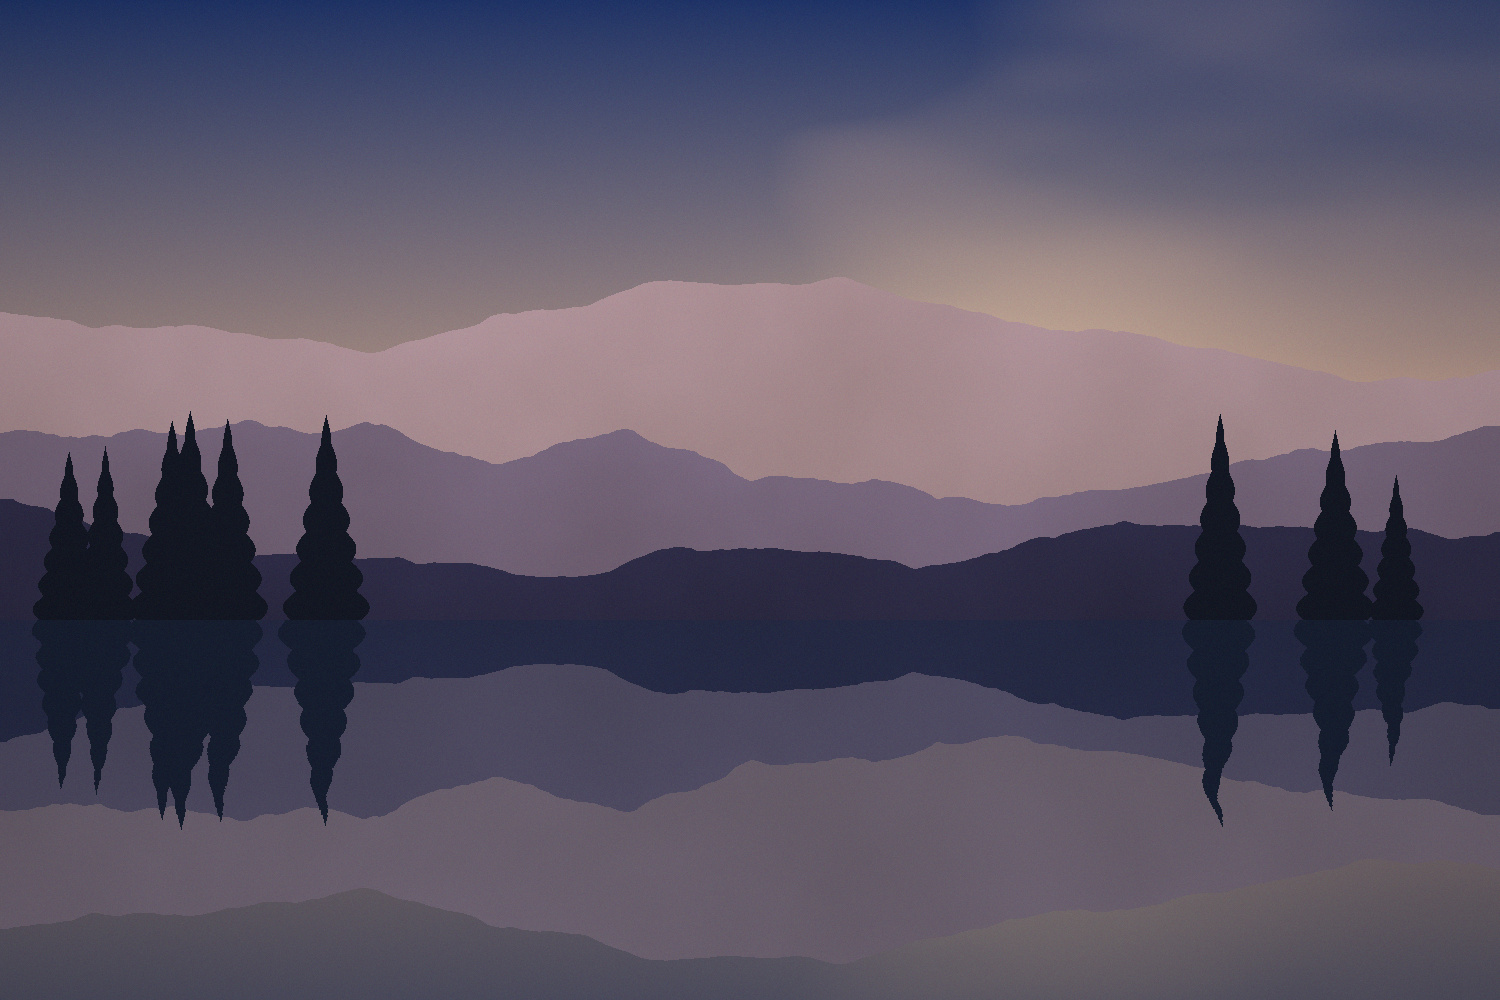
\includegraphics[width=4.5cm]{photo_original.jpg}};
    \draw[photo] (po.south west) rectangle (po.north east);
    \node[inner sep=0pt] (pc) at (12.1,3.95) {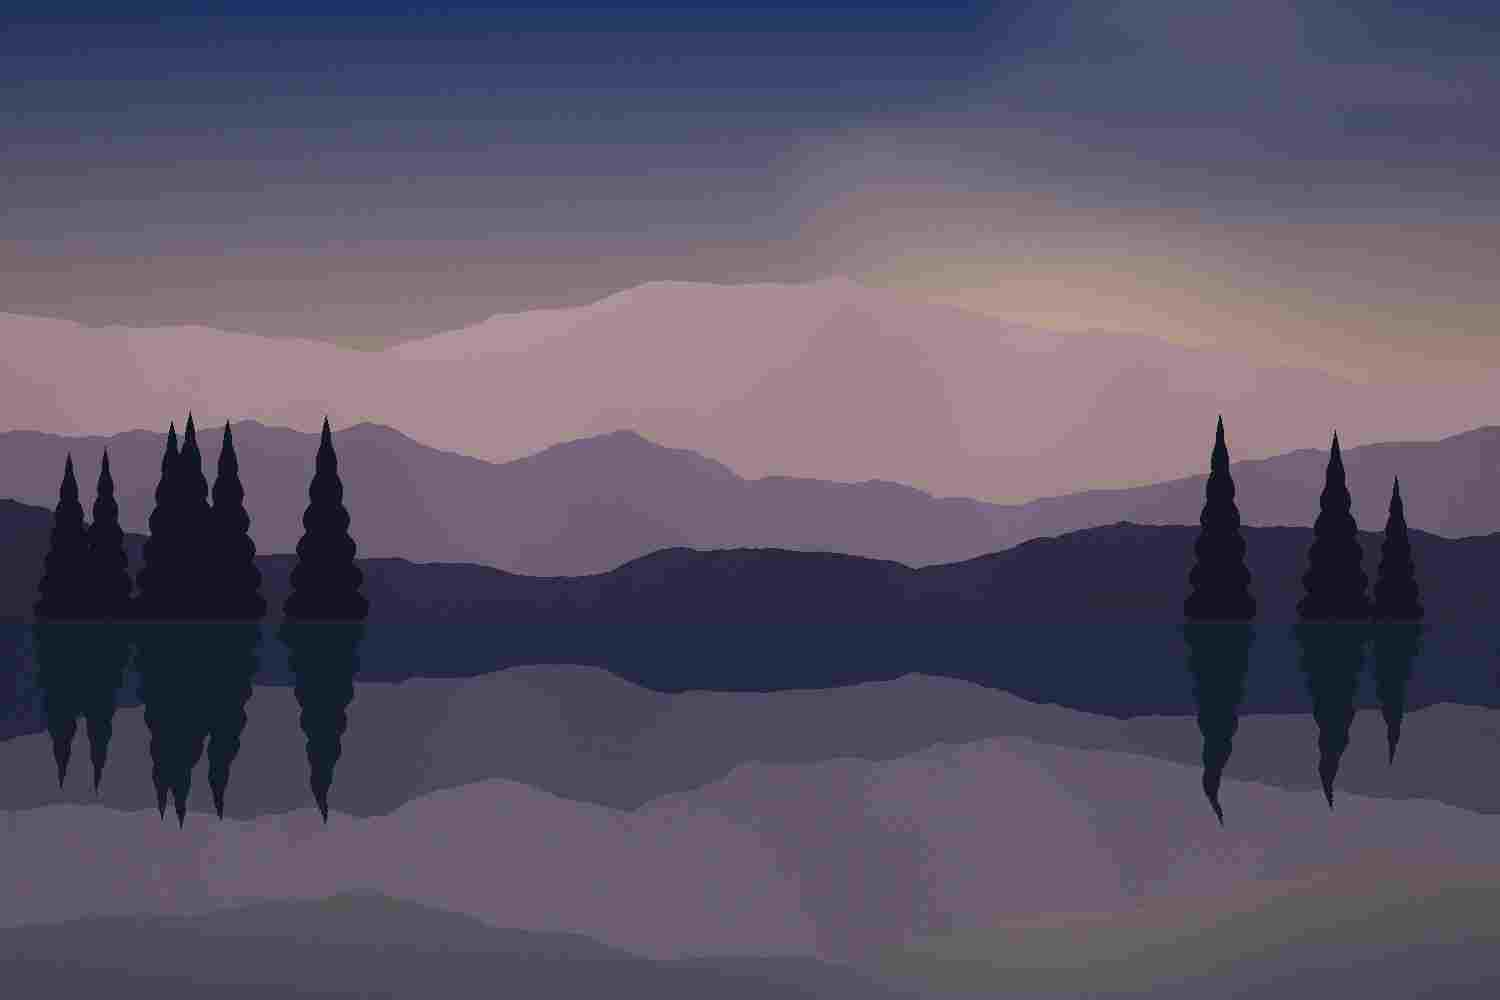
\includegraphics[width=4.5cm]{photo_compressed.jpg}};
    \draw[photo] (pc.south west) rectangle (pc.north east);
    \node[mystery,minimum width=1.9cm,minimum height=1.5cm,emphasis on=<2->] (pm) at (8,3.95) {?};
    \draw[arr] (po) -- (pm);
    \draw[arr] (pm) -- (pc);
    \node[lbl,anchor=north] at (po.south) {original \;\textbullet\; \textbf{2.8 MB}};
    \node[lbl,anchor=north] at (pc.south) {compressed \;\textbullet\; \textbf{180 KB} \;\textcolor{teal}{($\approx$15$\times$ smaller)}};

    \node[font=\normalsize,text=ink,align=center] at (8,1.3)
       {Compressed image is \textbf{\textcolor{deepteal}{15 times smaller}}};

  \end{scope}}


\end{canvas}
\end{frame}

% =================================================================
%  PAGE 3 — Enter the autoencoder
% =================================================================
\begin{frame}{Enter the Autoencoder}
\begin{canvas}
  \only<1-2>{%
    \node[inner sep=0pt] (po) at (3.3,4.5) {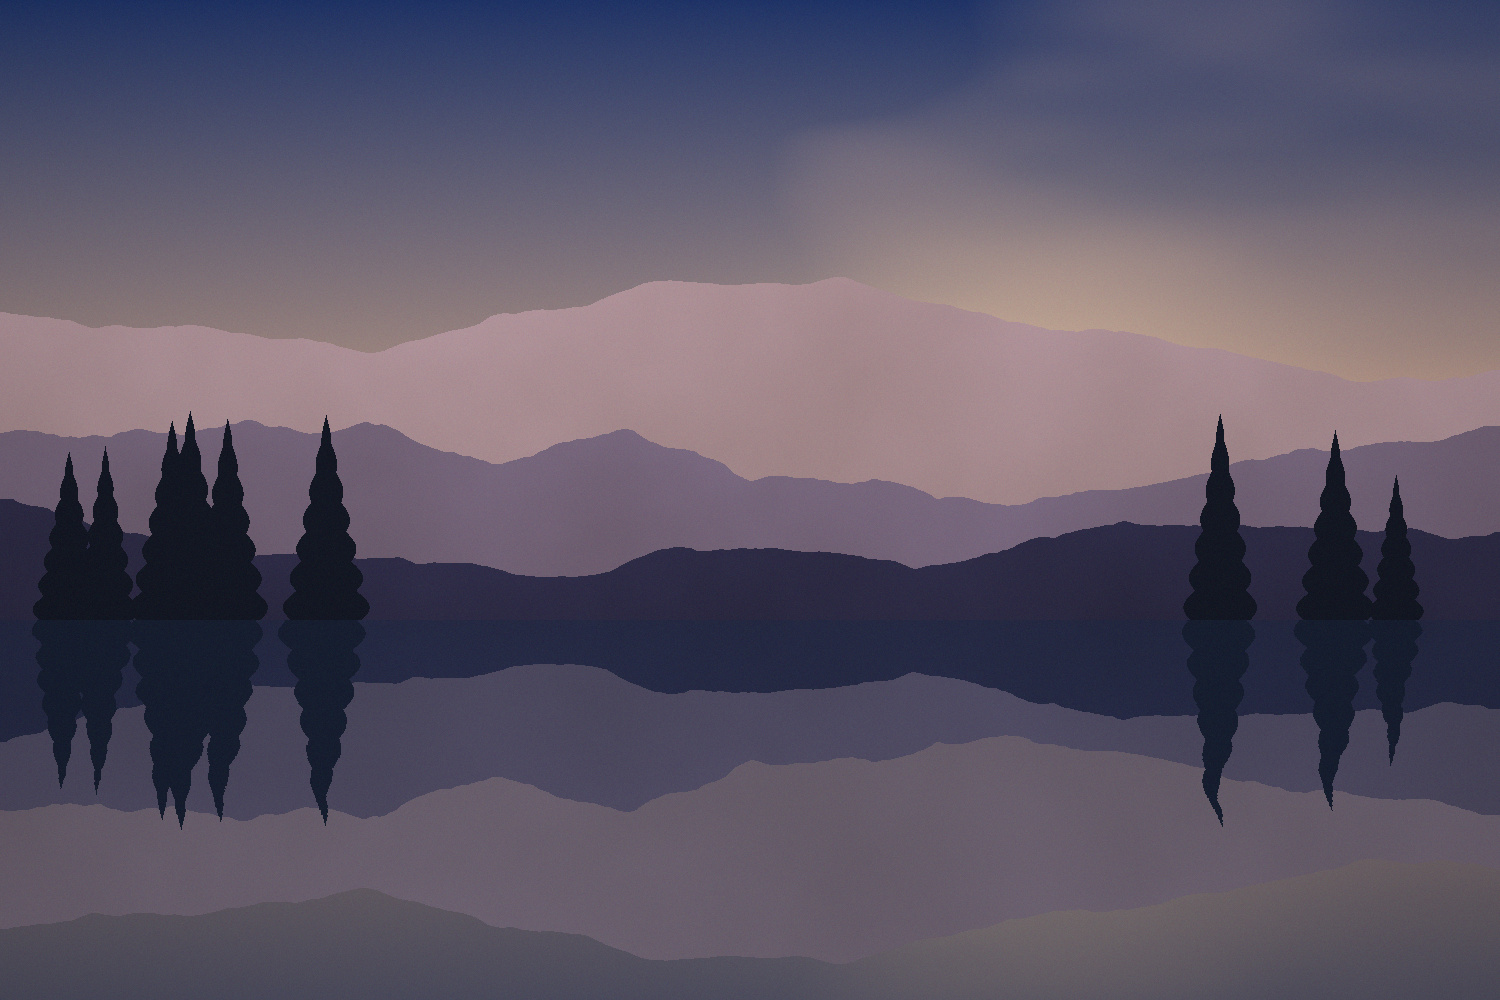
\includegraphics[width=3.9cm]{photo_original.jpg}};
    \draw[photo] (po.south west) rectangle (po.north east);
    \node[inner sep=0pt] (pc) at (12.7,4.5) {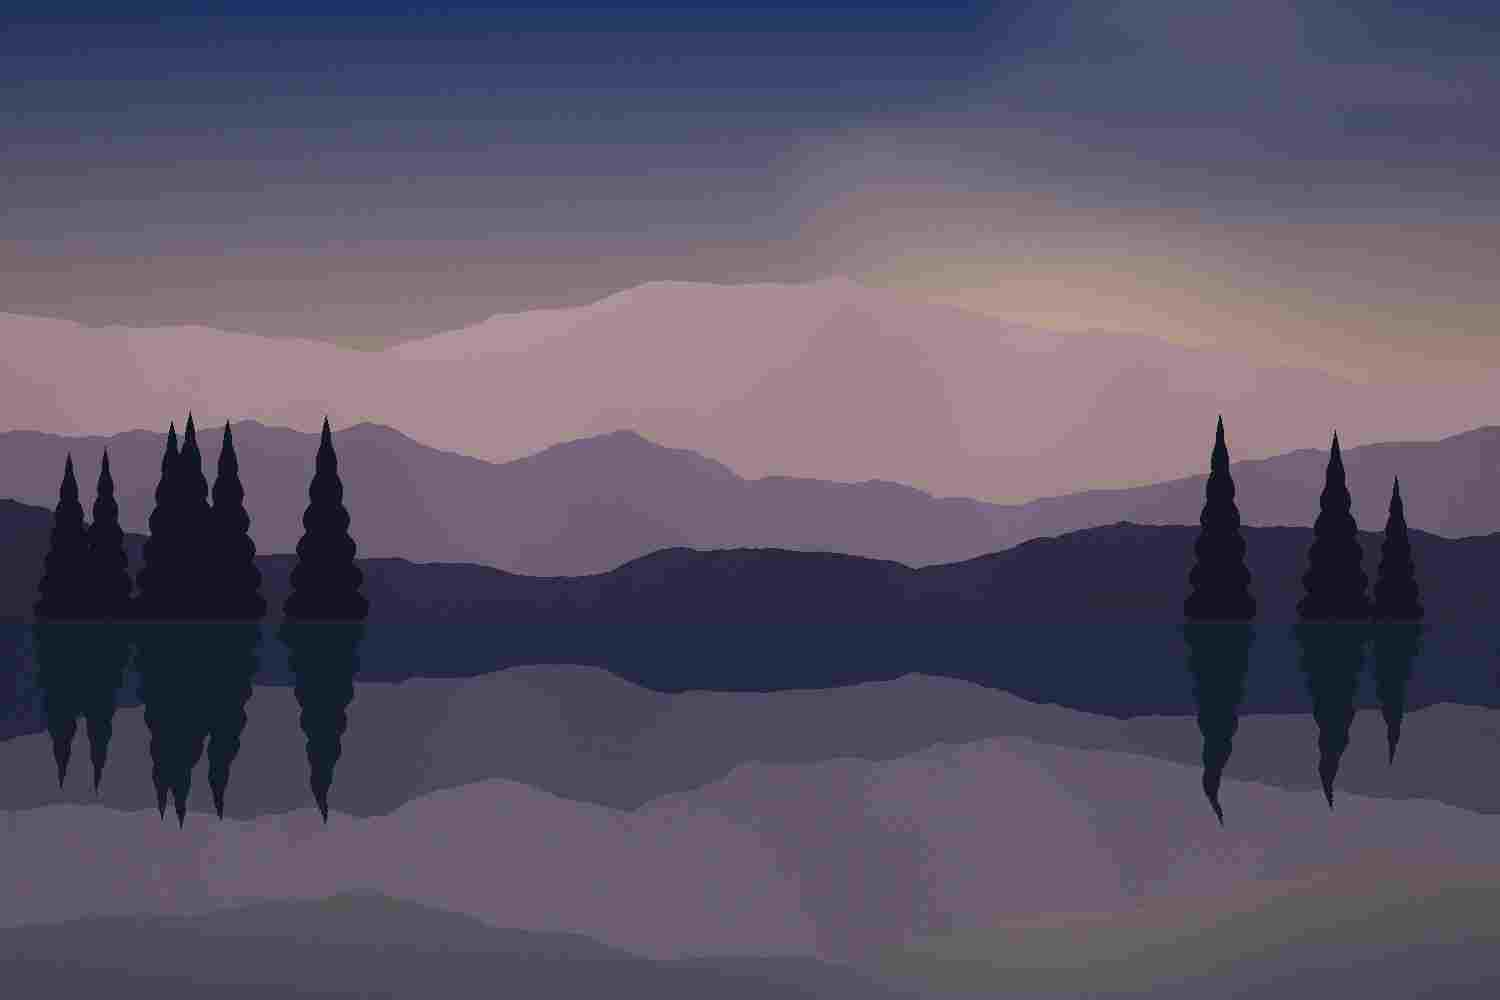
\includegraphics[width=3.9cm]{photo_compressed.jpg}};
    \draw[photo] (pc.south west) rectangle (pc.north east);
    \node[lbl,anchor=north] at (po.south) {2.8 MB};
    \node[lbl,anchor=north] at (pc.south) {180 KB};
    \draw[arr] (po) -- (8-1.95,4.5);
    \draw[arr] (8+1.95,4.5) -- (pc);

    \node[mystery,minimum width=3.9cm,minimum height=2.6cm,emphasis on=<1>,
          alt=<2>{draw=navy,line width=1pt}{}] (box) at (8,4.5) {};
    \node[visible on=<1>,text=deepteal,font=\fontsize{40}{40}\fontseries{eb}\selectfont] at (box) {?};

    \only<1>{\node[font=\large,text=ink,align=center] at (8,2.0)
       {What goes inside the \textbf{\textcolor{deepteal}{mysterious middle box}}?};}

    \begin{scope}[visible on=<2>]
      \node[text=navy,font=\large\fontseries{eb}\selectfont] at (8,5.3) {Autoencoder};
      \fill[steel!12] (6.55,4.85) -- (7.65,4.45) -- (7.65,3.95) -- (6.55,3.55) -- cycle;
      \draw[steel,line width=0.8pt] (6.55,4.85) -- (7.65,4.45) -- (7.65,3.95) -- (6.55,3.55) -- cycle;
      \fill[teal!10] (9.45,4.85) -- (8.35,4.45) -- (8.35,3.95) -- (9.45,3.55) -- cycle;
      \draw[teal,line width=0.8pt] (9.45,4.85) -- (8.35,4.45) -- (8.35,3.95) -- (9.45,3.55) -- cycle;
      \node[rectangle,fill=navy!8,draw=navy,line width=0.8pt,minimum width=0.42cm,minimum height=0.5cm,
            inner sep=0pt,font=\scriptsize,text=navy] at (8,4.2) {$z$};
      \draw[slate,line width=0.6pt,->,>={Stealth[length=1.3mm]}] (7.65,4.2) -- (7.79,4.2);
      \draw[slate,line width=0.6pt,->,>={Stealth[length=1.3mm]}] (8.21,4.2) -- (8.35,4.2);
      \node[font=\tiny,text=steel] at (7.0,3.35) {encoder};
      \node[font=\tiny,text=teal!80!black] at (9.0,3.35) {decoder};
    \end{scope}

    \node[visible on=<2>,font=\large,text=ink,align=center] at (8,2.0)
         {This box is exactly where \textbf{\textcolor{navy}{autoencoders}} come in.};
  }
  % ---------- step 3: big standalone autoencoder diagram ----------
  \begin{scope}[visible on=<3->]
    \node[draw=navy,line width=1.3pt,rounded corners=5pt,fill=white,
          minimum width=6.2cm,minimum height=4.13cm] (bigbox) at (8,4.7) {};
    \node[text=navy,font=\Large\fontseries{eb}\selectfont] at (8,5.97) {Autoencoder};

    \fill[steel!12] (5.69,5.26) -- (7.44,4.62) -- (7.44,3.83) -- (5.69,3.19) -- cycle;
    \draw[steel,line width=1.2pt] (5.69,5.26) -- (7.44,4.62) -- (7.44,3.83) -- (5.69,3.19) -- cycle;
    \fill[teal!10] (10.31,5.26) -- (8.56,4.62) -- (8.56,3.83) -- (10.31,3.19) -- cycle;
    \draw[teal,line width=1.2pt] (10.31,5.26) -- (8.56,4.62) -- (8.56,3.83) -- (10.31,3.19) -- cycle;
    \node[rectangle,fill=navy!8,draw=navy,line width=1.2pt,minimum width=0.67cm,minimum height=0.8cm,
          inner sep=0pt,font=\normalsize,text=navy] at (8,4.22) {$z$};
    \draw[slate,line width=1pt,->,>={Stealth[length=2mm]}] (7.44,4.22) -- (7.67,4.22);
    \draw[slate,line width=1pt,->,>={Stealth[length=2mm]}] (8.33,4.22) -- (8.56,4.22);
    \node[font=\normalsize,text=steel] at (6.41,2.87) {encoder};
    \node[font=\normalsize,text=teal!80!black] at (9.59,2.87) {decoder};
  \end{scope}

  \node[visible on=<3->,font=\large,text=ink,align=center] at (8,2.0)
       {A neural network that learns to \textcolor{steel}{\textbf{compress}} data and \textcolor{teal}{\textbf{reconstruct}} it};

  \node[visible on=<3->,lbl, font = \normalsize] at (8,1.45)
       {It has two main parts: \textcolor{steel}{\textbf{1. Encoder }} \textcolor{teal}{\textbf{2. Decoder}}};
\end{canvas}
\end{frame}

% =================================================================
%  PAGE 4 — Autoencoder architecture
% =================================================================
\begin{frame}{Autoencoder Architecture}
\begin{canvas}
  % layers: x positions and node counts
  \def\LA{4.3}\def\LB{6.05}\def\LC{7.95}\def\LD{9.85}\def\LE{11.6}
  \def\yc{4.45}

  % bottleneck band
  \draw[fill=navy!5,draw=navy!35,line width=0.6pt,dashed,rounded corners=4pt,visible on=<2->,focus on=<2>]
       (7.35,2.75) rectangle (8.55,6.15);
  \node[visible on=<2->,font=\scriptsize\bfseries,text=navy] at (7.95,5.85) {bottleneck};
  \node[visible on=<2->,font=\scriptsize,text=navy,align=center] at (7.95,3.05) {code $z$};

  % nodes
  \begin{scope}[visible on=<1->]
    \foreach \i in {1,...,5} \node[neuron,fill=steel!12,draw=steel,text=navy] (a\i) at (\LA,{\yc+(3-\i)*0.75}) {$x_{\i}$};
    \foreach \i in {1,...,3} \node[neuron,fill=steel!12,draw=steel] (b\i) at (\LB,{\yc+(2-\i)*0.75}) {};
    \foreach \i in {1,...,2} \node[neuron,fill=navy!8,draw=navy,text=navy] (c\i) at (\LC,{\yc+(1.5-\i)*0.8}) {$z_{\i}$};
    \foreach \i in {1,...,5} \foreach \j in {1,...,3} \draw[slate!45,line width=0.35pt] (a\i) -- (b\j);
    \foreach \i in {1,...,3} \foreach \j in {1,...,2} \draw[slate!45,line width=0.35pt] (b\i) -- (c\j);
    \node[inner sep=0pt] (xin) at (2.0,\yc) {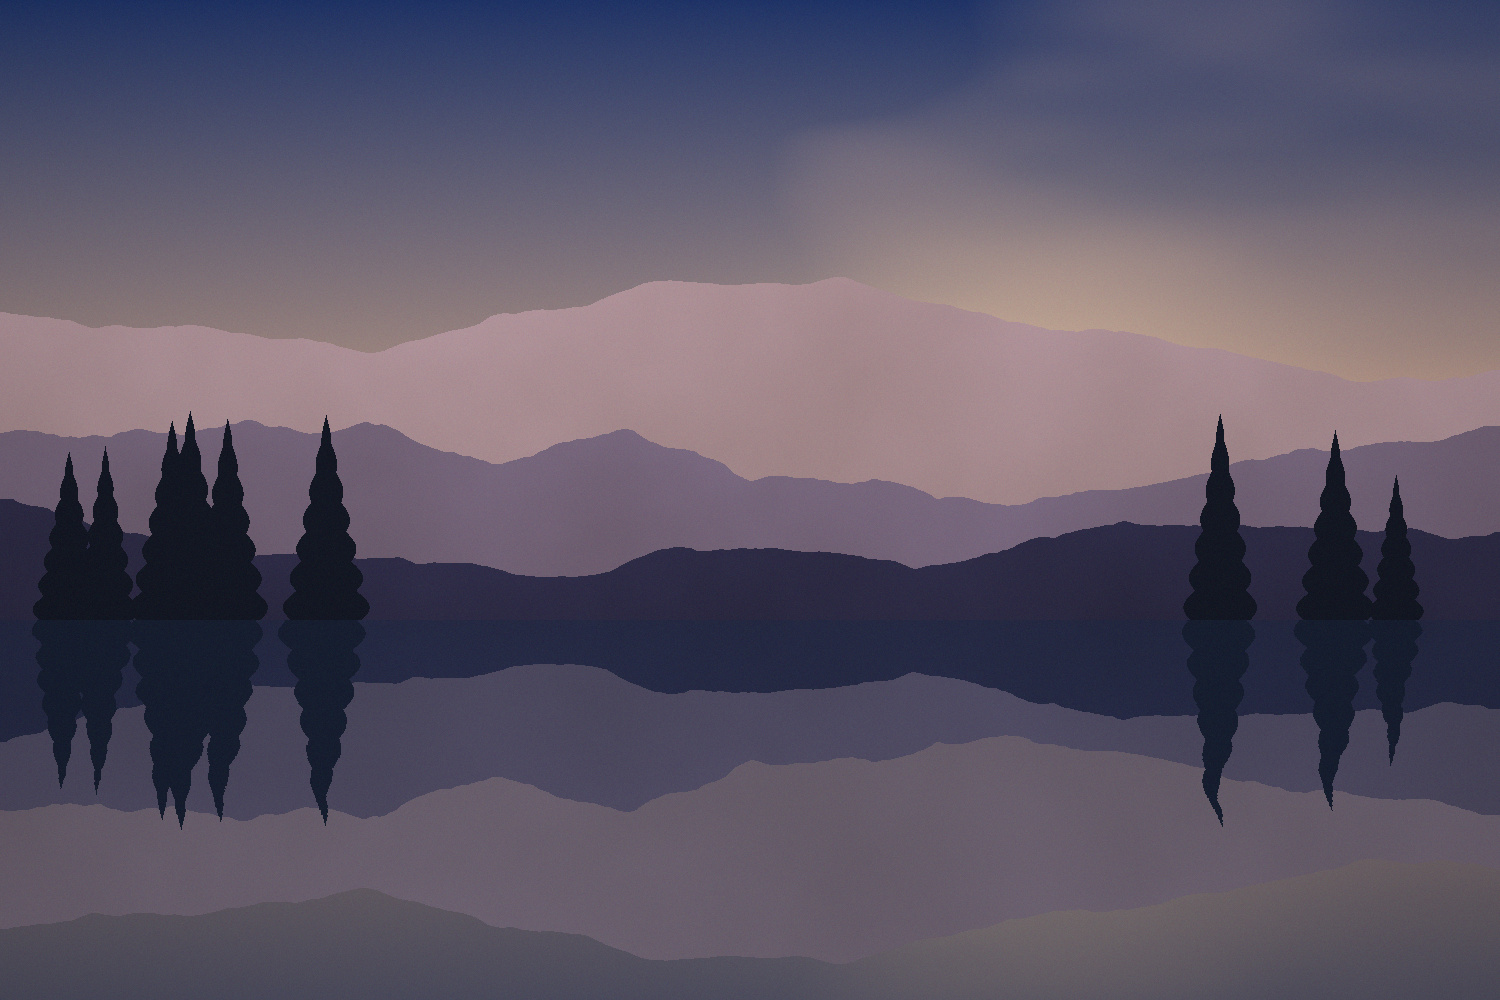
\includegraphics[width=2.1cm]{photo_original.jpg}};
    \draw[photo] (xin.south west) rectangle (xin.north east);
    \node[lbl,anchor=north] at (xin.south) {input $x$};
    \draw[arr] (xin.east) -- ++(0.9,0);
    \draw[decorate,decoration={brace,amplitude=6pt},steel,line width=0.8pt] (4.0,6.4) -- (7.4,6.4)
         node[midway,above=6pt,font=\footnotesize\bfseries,text=steel] {\ding{172}\; Encoder};
  \end{scope}
  \begin{scope}[visible on=<3->]
    \foreach \i in {1,...,3} \node[neuron,fill=teal!10,draw=teal] (d\i) at (\LD,{\yc+(2-\i)*0.75}) {};
    \foreach \i in {1,...,5} \node[neuron,fill=teal!10,draw=teal,text=teal!70!black] (e\i) at (\LE,{\yc+(3-\i)*0.75}) {$\hat{x}_{\i}$};
    \foreach \i in {1,...,2} \foreach \j in {1,...,3} \draw[slate!45,line width=0.35pt] (c\i) -- (d\j);
    \foreach \i in {1,...,3} \foreach \j in {1,...,5} \draw[slate!45,line width=0.35pt] (d\i) -- (e\j);
    \node[inner sep=0pt] (xout) at (13.9,\yc) {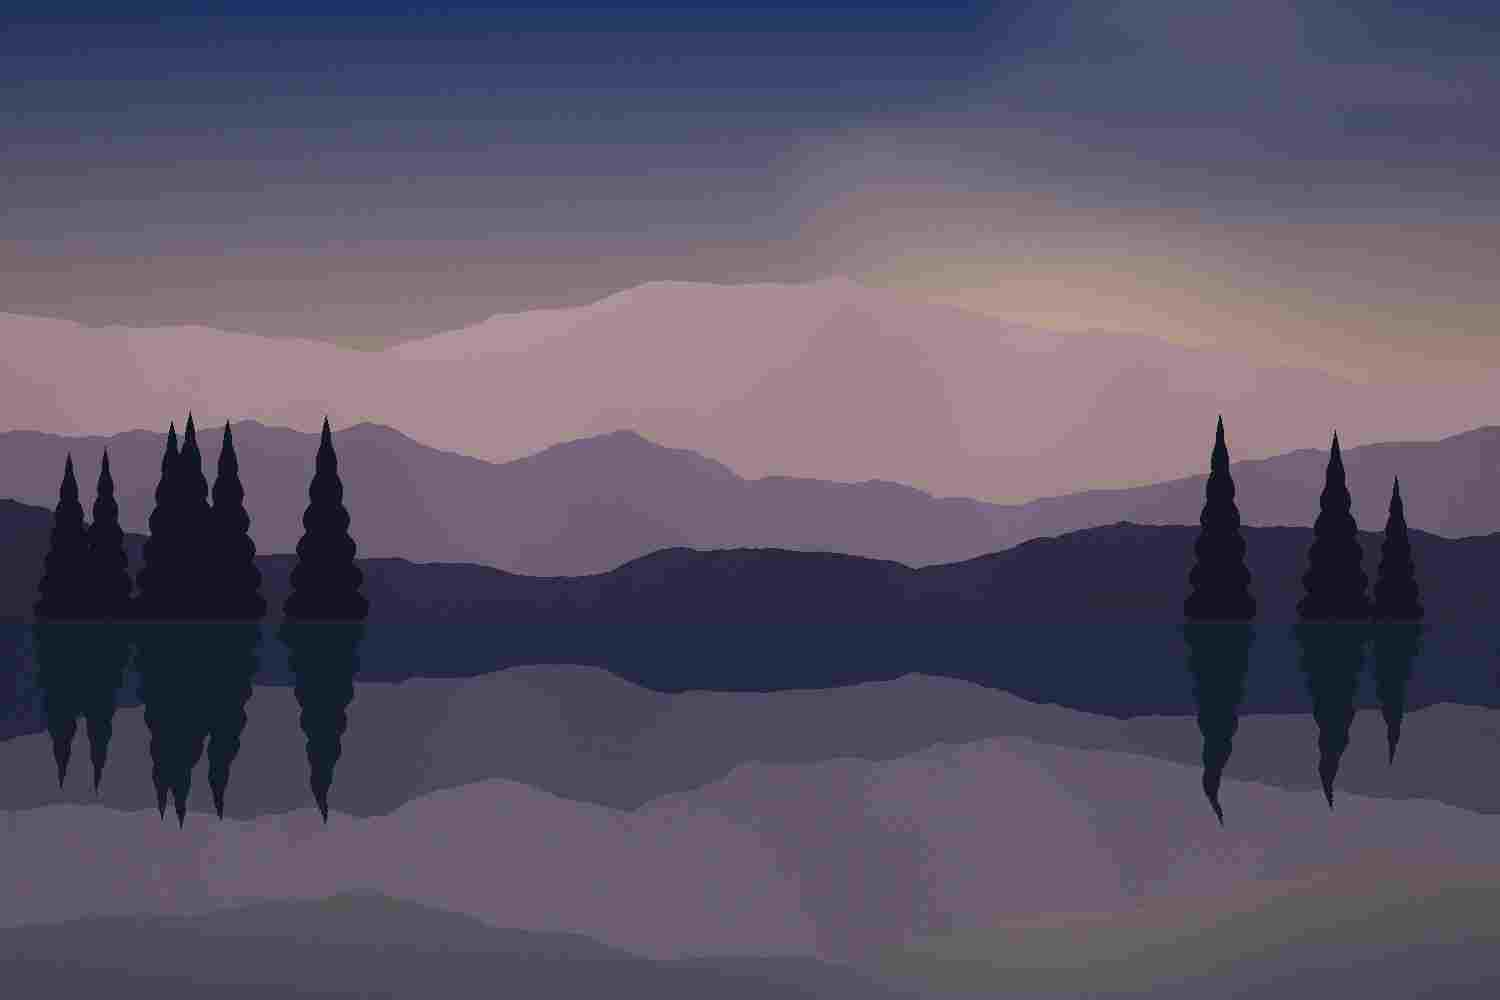
\includegraphics[width=2.1cm]{photo_compressed.jpg}};
    \draw[photo] (xout.south west) rectangle (xout.north east);
    \node[lbl,anchor=north] at (xout.south) {reconstruction $\hat{x}$};
    \draw[arr] (11.9,\yc) -- (xout.west);
    \draw[decorate,decoration={brace,amplitude=6pt},teal,line width=0.8pt] (8.5,6.4) -- (11.9,6.4)
         node[midway,above=6pt,font=\footnotesize\bfseries,text=teal!80!black] {\ding{173}\; Decoder};
  \end{scope}
  % redraw node layer on top of edges
  \begin{scope}[visible on=<1->]
    \foreach \i in {1,...,2} \node[neuron,fill=navy!8,draw=navy,text=navy] at (c\i) {$z_{\i}$};
  \end{scope}

  % explanation
  \node[font=\normalsize,text=ink,align=center,text width=13cm] at (8,1.55) {%
    \only<1>{The \textbf{\textcolor{steel}{encoder}} compresses the image, layer by layer, until it reaches the bottleneck.}%
    \only<2>{The \textbf{\textcolor{navy}{bottleneck}} allows only the \emph{essential} information to pass which is called \emph{\textcolor{navy}{latent code}}, represented in the \emph{\textcolor{navy}{latent space}} }%
    \only<3>{The \textbf{\textcolor{teal}{decoder}} uses that latent code to rebuild the image: \; $\hat{x}\approx x$.}};
\end{canvas}
\end{frame}
% =================================================================
%  PAGE 5 — Latent space: islands and gaps
% =================================================================
\begin{frame}{The Problem with Autoencoders}
\begin{canvas}
  \begin{scope}[shift={(4.65,4.1)}]
    \latentpanel
    \clusters{0}{1}
  \only<1,3>{\clusterlabels{1}}
  \only<2>{%
    \foreach \cx/\cy/\dx/\dy/\d in {-2.35/1.55/-0.95/0.25/0, -0.25/1.85/0.55/0.3/1, 2.20/1.20/0.2/0.8/7,
                                    -2.05/-1.35/0.9/-0.5/3, 0.60/-0.45/-0.8/-0.5/5, 2.40/-1.65/-0.15/-0.75/9}
      {\thumb[minimum size=0.62cm,draw=teal,line width=1pt,fill=teal!10,
              font=\normalsize\fontseries{eb}\selectfont,text=teal!80!black]{\cx+\dx,\cy+\dy}{\d}}
  }
    % step 2: one dot = one image
    \begin{scope}[visible on=<1>]
      \draw[sky,line width=0.9pt] (2.2,1.2) circle (0.14);
      \draw[sky,line width=0.6pt] (2.33,1.15) -- (2.85,0.05);
      \node[fill=white,draw=sky,line width=0.9pt,rounded corners=3pt,font=\normalsize,text=sky!70!black,
            inner sep=5pt,anchor=west] at (2.95,-0.05) {\textbf{1 dot = 1 image}};
    \end{scope}
    % step 3: highlight gaps
    \begin{scope}[visible on=<3->]
      \foreach \x/\y/\r in {-1.25/0.3/0.55, 1.3/0.2/0.5, -0.5/-1.95/0.45, 1.0/2.2/0.32, 3.1/-0.1/0.4}
        \draw[slate,line width=0.6pt,dash pattern=on 2pt off 1.6pt] (\x,\y) circle (\r);
      \node[font=\scriptsize\itshape,text=slate] at (-1.25,0.3) {empty};
      \node[font=\scriptsize\itshape,text=slate] at (1.3,0.2) {empty};
    \end{scope}
  \end{scope}

  % right-hand explanation
  \node[anchor=north west,text width=6.2cm,align=left,font=\normalsize,text=ink] at (8.95,6.9) {%
    Here in this bottleneck space, each point is exactly \textbf{one image} after compression};
  \node[anchor=north west,text width=6.2cm,align=left,font=\normalsize,text=ink,visible on=<2->] at (8.95,5.2) {%
    Notice how similar images form separate \textbf{\textcolor{navy}{islands}}, such as 0, 1, 5, 7, and 9};
  \node[anchor=north west,text width=6.2cm,align=left,font=\normalsize,text=ink,visible on=<3->] at (8.95,3.5) {%
     There are lots of \textbf{\textcolor{teal}{empty spaces}} between them. The decoder has not seen training examples from these regions.};
\end{canvas}
\end{frame}

% =================================================================
%  PAGE 6 — Sampling from a gap
% =================================================================
\begin{frame}{What Lives in the Gaps?}
\begin{canvas}
  \begin{scope}[shift={(4.65,4.1)}]
    \latentpanel
    \clusters{0}{1}
        \foreach \cx/\cy/\dx/\dy/\d in {-2.35/1.55/-0.95/0.25/0, -0.25/1.85/0.55/0.3/1, 2.20/1.20/0.2/0.8/7,
                                    -2.05/-1.35/0.9/-0.5/3, 0.60/-0.45/-0.8/-0.5/5, 2.40/-1.65/-0.15/-0.75/9}
      {\thumb[minimum size=0.62cm,draw=teal,line width=1pt,fill=teal!10,
              font=\normalsize\fontseries{eb}\selectfont,text=teal!80!black]{\cx+\dx,\cy+\dy}{\d}}
    % A: inside an island    
    \draw[navy,line width=1pt] (2.2,1.2) circle (0.16);
    \draw[navy,line width=0.6pt] (2.34,1.14) -- (3.15,0.7);
    \node[fill=white,draw=navy,line width=0.9pt,rounded corners=3pt,font=\normalsize,text=navy,
          inner sep=4pt,anchor=west] at (3.25,0.7) {\textbf{A}};
    % B: in an empty region
    \begin{scope}[visible on=<2->]
      \draw[teal,line width=0.6pt,dash pattern=on 2pt off 1.6pt] (-1.25,0.3) circle (0.5);
      \node[star,star points=5,star point ratio=2.3,fill=navy,inner sep=1.4pt] at (-1.25,0.3) {};
      \draw[navy,line width=0.6pt] (-0.75,0.3) -- (-0.35,0.3);
      \node[fill=white,draw=navy,line width=0.9pt,rounded corners=3pt,font=\normalsize,text=navy!80!black,
            inner sep=4pt,anchor=west] at (-0.25,0.3) {\textbf{B}};
    \end{scope}
  \end{scope}

  % right: decode A and B
  \tikzset{smalldec/.style={dec,minimum width=1.1cm,minimum height=1.0cm,inner sep=1pt,font=\tiny\bfseries}}
  \node[font=\footnotesize,text=navy,anchor=west] at (8.95,6.95) {\textbf{A}\; point inside an island};
  \node[smalldec] (dA) at (11.2,5.95) {Decoder};
  \draw[arr] (9.3,5.95) -- (dA.west);
  \thumb[minimum size=1.1cm,font=\huge\fontseries{eb}\selectfont]{13.25,5.95}{7}
  \draw[arr] (dA.east) -- (12.65,5.95);
  \node[font=\footnotesize,text=navy,anchor=north] at (13.25,5.33) {\cmark\ a clear ``7''};


  \begin{scope}[visible on=<2->]
    \node[font=\footnotesize,text=teal!80!black,anchor=west] at (8.95,3.6) {\textbf{B}\; random point from an empty gap};
    \node[smalldec] (dB) at (11.2,2.6) {Decoder};
    \draw[arr] (9.3,2.6) -- (dB.west);
      \thumb[minimum size=1.1cm,font=\huge\fontseries{eb}\selectfont]{13.25,2.75}{?}
    \garbled{13.25,2.6}{1.1}
    \draw[arr] (dB.east) -- (12.65,2.6);
    \node[font=\footnotesize,text=teal!80!black,anchor=north] at (13.25,1.98) {\xmark\ meaningless};
  \end{scope}

\end{canvas}
\end{frame}

% =================================================================
%  PAGE — A new idea
% =================================================================
\begin{frame}{The Key Insight}
\begin{canvas}
  % ---------- the question ----------
  \fill[ink!8,rounded corners=6pt] (2.95,4.0) rectangle (13.15,6.05);
  \draw[steel,line width=1.2pt,rounded corners=6pt,top color=steel!12,bottom color=white]
       (2.8,4.15) rectangle (13.0,6.2);
  \node[text width=8.8cm,align=center,font=\large,text=ink] at (7.9,5.18) {%
    Instead of storing each image as one exact point, what if every image were represented as a \textbf{\textcolor{steel}{distribution}}?};

  % ---------- the answer ----------
      \begin{scope}[visible on=<2->]
    \fill[ink!10,rounded corners=6pt] (2.95,1.85) rectangle (13.15,3.6);
    \draw[teal,line width=1.4pt,rounded corners=6pt,top color=teal!18,bottom color=white]
         (2.8,2.0) rectangle (13.0,3.75);
    \node[text width=9.2cm,align=center,font=\large\bfseries,text=teal] at (7.9,2.88) {%
      That's the core idea behind the \textcolor{teal!60!navy}{Variational Autoencoder (VAE)}};
  \end{scope}
\end{canvas}
\end{frame}
% =================================================================
%  PAGE 7 — From points to distributions
% =================================================================
\begin{frame}{From Points to Distributions}
\begin{canvas}
  \begin{scope}[shift={(4.65,4.1)}]
    \latentpanel
    \begin{scope}
      \clip (-3.7,-2.95) rectangle (3.7,2.95);
      \only<1>{\clusters{0}{1}}
      \only<2>{\clusters{0.24}{1}}
      \only<3->{\clusters{0.42}{0.7}}
    \end{scope}
    \only<1-2>{\clusterlabels{1}}
    \only<3->{%
      \node[star,star points=5,star point ratio=2.3,fill=teal,inner sep=1.4pt] (new) at (-0.55,0.35) {};
      \draw[teal,line width=0.6pt] (new) -- (-2.2,-2.45)
        node[fill=white,draw=teal,rounded corners=2pt,inner sep=2.5pt,font=\scriptsize,text=teal!80!black,anchor=north west]
        at (-3.55,-2.1) {sampled point $\rightarrow$ plausible image};}
  \end{scope}

  % ---------- morph: one image -> one point / one cloud (slides 1,2 only) ----------
  \only<1,2>{%
    \thumb[minimum size=0.9cm,font=\LARGE\fontseries{eb}\selectfont]{9.6,5.05}{3}
    \node[lbl] at (9.6,4.35) {one image};
    \draw[arr] (10.15,5.05) -- (11.35,5.05);
    \node[lbl,font=\scriptsize] at (10.75,5.3) {encode};
  }
  \coordinate (P) at (12.95,5.05);
  \only<1>{%
    \fill[navy] (P) circle (0.09);
    \node[lbl,text=navy] at ($(P)+(0,-0.7)$) {one exact point};}
  \only<2>{%
    \fill[navy,opacity=0.07] (P) ellipse (1.25 and 0.72);
    \fill[navy,opacity=0.09] (P) ellipse (0.85 and 0.5);
    \fill[navy,opacity=0.12] (P) ellipse (0.48 and 0.28);
    \draw[navy!60,line width=0.5pt,dashed] (P) ellipse (1.25 and 0.72);
    \pgfmathsetseed{9}
    \foreach \k in {1,...,26}{
      \pgfmathsetmacro\rr{min(1.8,sqrt(-2*ln(max(rnd,0.01))))}
      \pgfmathsetmacro\tt{360*rnd}
      \fill[navy!70] ($(P)+({0.45*\rr*cos(\tt)},{0.26*\rr*sin(\tt)})$) circle (0.035);}
    \fill[navy] (P) circle (0.07);
    \draw[steel,line width=0.7pt,<->,>={Stealth[length=1.2mm]}] (P) -- ++(0.85,0)
         node[midway,above=-1pt,font=\scriptsize,text=steel] {$\bm{\sigma}$};
    \node[font=\scriptsize,text=navy] at ($(P)+(-0.2,-0.2)$) {$\bm{\mu}$};
    \node[lbl,text=navy] at ($(P)+(0,-0.98)$) {a small cloud \; $\mathcal{N}(\bm{\mu},\bm{\sigma}^2)$};}

  % ---------- slide 3: text on top ----------
  \only<3>{%
    \node[anchor=north west,text width=5.9cm,align=left,font=\footnotesize,text=ink] at (9.15,6.9) {%
      Notice, the distributions overlap, which \textbf{reduces empty gaps}.\\[10pt]As a result, we can choose a new point from that area and it will still decode into a meaningful image.};
  }

    % ---------- slide 3: flowchart below the text ----------
  \only<3>{%
    \node[draw=teal,line width=0.6pt,rounded corners=3pt,fill=white,minimum width=2.0cm,minimum height=0.75cm,
          font=\footnotesize,text=teal!80!black] (fs1) at (9.6,3.1) {Sample point};
    \node[dec,minimum width=1.6cm,minimum height=0.9cm,inner sep=1pt,font=\small\bfseries] (fs2) at (12.3,3.1) {Decoder};
    \node[draw=slate!50,line width=0.5pt,fill=white,minimum size=1.0cm,inner sep=0pt,text=teal!70!black,
          font=\huge\fontseries{eb}\selectfont] (fs3) at (14.6,3.1) {\checkmark};
    \draw[arr] (fs1) -- (fs2);
    \draw[arr] (fs2) -- (fs3);
    \node[lbl,anchor=north,text=teal!80!black] at (14.6,2.35) {Meaningful\\image};
  }

  % ---------- highlight chips ----------
  \node[chip,draw=teal,anchor=west,text width=5.55cm,inner xsep=5pt,align=left,visible on=<2>,line width=1.1pt] at (9.1,2.9)
       {\textbf{\textcolor{teal}{VAE:}} one image $\rightarrow$ one \textbf{distribution}};

  \only<2>{%
    \node[anchor=north west,text width=5.9cm,align=left,font=\footnotesize,text=ink] at (9.15,2.55) {%
      Each image now occupies a \textbf{small area}.};
  }
\end{canvas}
\end{frame}


% =================================================================
%  PAGE 8 — Smile: value vs distribution  (senior slide 27)
% =================================================================
\begin{frame}{One Image, One Distribution}
\begin{canvas}
  \def\xa{5.0}\def\xb{11.2}\def\W{4.2}
  % headers
  \node[font=\footnotesize\bfseries,text=ink] at (\xa,7.1) {Smile (discrete value)};
  \node[chip,draw=steel,font=\scriptsize] at (\xa,6.62) {$\rightarrow$ \textbf{\textcolor{steel}{Autoencoder}}: a single point};
  \begin{scope}[visible on=<2->]
    \node[font=\footnotesize\bfseries,text=ink] at (\xb,7.1) {Smile (probability distribution)};
    \node[chip,draw=teal,font=\scriptsize,line width=1.1pt] at (\xb,6.62) {$\rightarrow$ \textbf{\textcolor{teal}{Variational Autoencoder}}: a distribution};
    \node[font=\footnotesize\itshape,text=slate] at (8.1,3.8) {vs.};
  \end{scope}
  \node[lbl,rotate=90,font=\scriptsize] at (0.95,3.8) {each row = one image};

  \foreach \y/\s/\skin/\hair/\st/\bg/\shirt/\m/\sg/\h in {
      5.72/-0.5/teal!28!white/teal!75!ink/0/steel!10/sky!45/-0.55/0.26/0.62,
      4.42/0.05/teal!45!white/ink!85/1/slate!12/slate!55/0.0/0.42/0.42,
      3.12/0.6/teal!85!ink/ink/2/teal!12/teal!45/0.5/0.17/0.86,
      1.82/0.9/teal!55!white/slate!55!ink/3/navy!8/steel!60/0.78/0.1/0.95}{
    \face{2.05,\y}{1.02}{\s}{\skin}{\hair}{\st}{\bg}{\shirt}
    \numline{\xa,\y-0.3}{\W}
    \fill[navy] (\xa+\m*\W/2,\y-0.3) circle (0.085);
    \begin{scope}[visible on=<2->]
      \numline{\xb,\y-0.3}{\W}
      \gauss{\xb,\y-0.3}{\W}{\m}{\sg}{\h}
    \end{scope}}
\end{canvas}
\end{frame}

% =================================================================
%  PAGE 9 — Latent attributes as distributions  (senior slide 28)
% =================================================================
\begin{frame}{VAE Simplified: Latent Attributes}
\begin{canvas}
  \def\yc{4.45}
  \person{1.95,\yc}{1.45}
  \node[lbl,anchor=north] at (1.95,3.5) {input $x$};
  \node[enc,minimum width=2.1cm,minimum height=1.3cm,visible on=<1->,focus on=<1>] (en) at (4.25,\yc) {Encoder};
  \node[lbl,visible on=<1->] at (4.25,3.15) {$q_\phi(z\mid x)$};
  \draw[arr] (2.8,\yc) -- (en.west);

  % latent attribute panel
  \begin{scope}[visible on=<2->]
    \draw[slate!45,line width=0.6pt,rounded corners=8pt,fill=white] (5.75,2.1) rectangle (10.25,7.2);
    \draw[arr] (en.east) -- (5.7,\yc);
    \foreach \y/\name/\m/\sg/\h in {6.75/Smile/0.2/0.18/0.42, 5.9/Skin tone/0.05/0.25/0.34, 5.05/Gender/-0.45/0.16/0.46,
                                    4.2/Beard/0.7/0.12/0.52, 3.35/Glasses/-0.35/0.14/0.5, 2.5/Hair colour/0.05/0.12/0.52}{
      \node[anchor=east,font=\scriptsize,text=ink] at (7.3,\y) {\name};
      \numline{8.75,\y-0.05}{2.4}
      \gauss{8.75,\y-0.05}{2.4}{\m}{\sg}{\h}}
    \node[lbl] at (8.0,1.75) {latent attributes: one distribution each};
  \end{scope}

  \begin{scope}[visible on=<3->]
    \node[dec,minimum width=2.1cm,minimum height=1.3cm,focus on=<3>] (de) at (11.75,\yc) {Decoder};
    \node[lbl] at (11.75,3.15) {$p_\theta(x\mid z)$};
    \draw[arr] (10.3,\yc) -- (de.west);
    \person{14.0,\yc}{1.45}
    \node[lbl,anchor=north] at (14.0,3.5) {reconstruction $\hat{x}$};
    \draw[arr] (de.east) -- (13.2,\yc);
  \end{scope}
\end{canvas}
\end{frame}

% =================================================================
%  PAGE 10 — Sample -> reconstruct  (senior slide 29)
% =================================================================
\begin{frame}{VAE Simplified: Sampling and Decoding}
\begin{canvas}
  % compact latent distributions with two samples
  \draw[slate!45,line width=0.6pt,rounded corners=8pt,fill=white] (0.95,1.85) rectangle (4.95,7.15);
  \foreach \y/\name/\m/\sg/\h/\a/\b in {6.7/Smile/0.2/0.18/0.42/0.23/0.17, 5.85/Skin tone/0.05/0.25/0.34/0.02/0.28,
                                        5.0/Gender/-0.15/0.16/0.46/-0.18/-0.11, 4.15/Beard/0.7/0.12/0.52/0.71/0.66,
                                        3.3/Glasses/-0.15/0.14/0.5/-0.19/-0.14, 2.45/Hair colour/0.3/0.12/0.52/0.33/0.26}{
    \node[anchor=west,font=\tiny,text=ink] at (1.05,\y+0.3) {\name};
    \numline{3.25,\y-0.05}{2.6}
    \gauss{3.25,\y-0.05}{2.6}{\m}{\sg}{\h}
    \begin{scope}[visible on=<1->]
      \fill[navy] (3.25+\a*1.3,\y-0.05) circle (0.06);
    \end{scope}
    \begin{scope}[visible on=<1->]
      \fill[teal] (3.25+\b*1.3,\y+0.08) circle (0.06);
    \end{scope}}
  \node[lbl] at (2.95,1.6) {latent distributions};

  % sampled attribute lists
  \foreach \yy/\c/\tag/\vals in {5.55/navy/A/{0.23,0.02,$-$0.18,0.71,$-$0.19,0.33},
                                  3.05/teal/B/{0.17,0.28,$-$0.11,0.66,$-$0.14,0.26}}{
    \begin{scope}[visible on=<2->]
      \draw[arr] (5.05,\yy) -- (6.25,\yy) node[midway,above,font=\scriptsize,text=\c] {sample \tag};
      \draw[\c!60,line width=0.6pt,rounded corners=4pt,fill=white] (6.3,\yy-1.02) rectangle (8.75,\yy+1.02);
      \foreach \v [count=\i] in \vals {
        \pgfmathsetmacro\ly{\yy+0.85-(\i-1)*0.34}
        \node[anchor=west,font=\tiny,text=slate] at (6.4,\ly)
             {\ifcase\i\or Smile\or Skin tone\or Gender\or Beard\or Glasses\or Hair colour\fi};
        \node[anchor=east,font=\tiny\bfseries,text=\c] at (8.65,\ly) {\v};}
    \end{scope}
    \begin{scope}[visible on=<3->]
      \node[dec,minimum width=1.3cm,minimum height=1.05cm,font=\scriptsize\bfseries] (d\tag) at (10.35,\yy) {Decoder};
      \draw[arr] (8.8,\yy) -- (d\tag.west);
      \draw[arr] (d\tag.east) -- (11.75,\yy);
    \end{scope}}
  \begin{scope}[visible on=<3->]
    \face{12.45,5.55}{1.2}{0.85}{teal!55!white}{slate!55!ink}{3}{steel!10}{steel!60}
    \face{12.45,3.05}{1.2}{0.6}{teal!55!white}{slate!55!ink}{3}{steel!10}{steel!60}
    \draw[slate,line width=0.6pt,<->,>={Stealth[length=1.3mm]}] (12.45,4.8) -- (12.45,3.8);
    \node[anchor=west,text width=2.25cm,align=left,font=\scriptsize,text=ink] at (13.2,4.3)
         {\textbf{same person}, tiny natural variations};
    \draw[fill=slate!7,draw=navy!40,line width=0.6pt,rounded corners=4pt] (6.3,0.98) rectangle (15.05,1.88);
    \node[font=\footnotesize,text=ink,align=center] at (10.67,1.43)
         {We expect an \textbf{accurate reconstruction} for \emph{any} sample\\ drawn from the latent distributions.};
  \end{scope}
\end{canvas}
\end{frame}
\endgroup

% #################################################################
%  PART 2  (from part2/part2_final.tex, unchanged)
%  Wrapped in a group: its colours, styles, macros and templates
%  apply only to its own slides.
% #################################################################
\begingroup
\graphicspath{{assets/part2/}}
\renewcommand{\familydefault}{\rmdefault}

% ---------- Your Theme Palette ----------
\definecolor{navy}{HTML}{002B55}
\definecolor{steel}{HTML}{4D6FAD}
\definecolor{sky}{HTML}{5DADF5}
\definecolor{teal}{HTML}{3F8C8A}
\definecolor{slate}{HTML}{5B6475}
\definecolor{paper}{HTML}{FBFAF7}
\definecolor{ink}{HTML}{1C2233}
\colorlet{deepteal}{navy!55!teal}

% ---------- Beamer Theme ----------
\setbeamercolor{background canvas}{bg=paper}
\setbeamercolor{normal text}{fg=ink}
\setbeamercolor{alerted text}{fg=teal}
\setbeamercolor{structure}{fg=navy}
\setbeamertemplate{navigation symbols}{}

\setbeamertemplate{background}{
  \begin{tikzpicture}[remember picture,overlay,shift={(current page.south west)}]
    \clip (0,0) rectangle (16,9);
  \end{tikzpicture}
}

\setbeamertemplate{frametitle}{%
  \begin{tikzpicture}[remember picture,overlay,shift={(current page.north west)}]
    \fill[navy] (0,0) rectangle (16,-1.05);
   
    \node[anchor=west,text=white,font=\fontseries{eb}\selectfont\Large] at (0.72,-0.525)
      {\insertframetitle};
  \end{tikzpicture}
  \vspace*{0.78cm}}

\setbeamertemplate{footline}{%
  \begin{tikzpicture}[remember picture,overlay,shift={(current page.south west)}]
    \node[anchor=west,font=\scriptsize,text=steel] at (0.72,0.32)
      {Variational Autoencoder \;\textcolor{slate!60}{|}\; CSE200};
    \node[anchor=east,font=\scriptsize\bfseries,text=steel] at (15.3,0.32)
      {\insertframenumber/\inserttotalframenumber};
  \end{tikzpicture}}

% ---------- Helpers ----------
\newenvironment{canvas}
  {\begin{tikzpicture}[remember picture,overlay,shift={(current page.south west)}]}
  {\end{tikzpicture}}

\tikzset{
  >={Stealth[length=2mm]},
  fwd/.style={->,line width=0.8pt,draw=ink},
  bigarrow/.style={fill=teal!35,draw=teal!80!black,line width=0.8pt},
  outline/.style={draw=teal,line width=1.55pt,fill=teal!8,opacity=0.18},
  box/.style={draw=navy,line width=1.25pt,rounded corners=5pt,fill=navy!4},
  hlt/.style={draw=teal,line width=1.55pt,fill=teal!8,opacity=0.18}
}


% ---------- Senior-style VAE diagram in your theme ----------
% Argument: input / encoder / latent / decoder / output / none
% Argument: input / encoder / latent / decoder / output / none

\newcommand{\VAEDiagram}[1]{

\begin{scope}[shift={(0.65,4.72)},scale=0.96]

  % =========================================================
  % INPUT x
  % =========================================================
  \fill[steel!18] (0.25,-1.00) rectangle (0.72,1.00);
  \draw[navy,line width=0.9pt] (0.25,-1.00) rectangle (0.72,1.00);
  \node[font=\scriptsize,text=navy] at (0.485,0) {$x$};

  % input -> encoder
  \draw[fwd] (0.72,0) -- (1.12,0);


  % =========================================================
  % ENCODER
  % =========================================================
  \node[
    trapezium,
    trapezium stretches=true,
    shape border rotate=270,
    minimum width=2.05cm,
    minimum height=1.65cm,
    draw=steel,
    line width=0.9pt,
    fill=steel!18,
    text=navy,
    font=\scriptsize
  ] (enc) at (1.95,0) {$h_{\phi}(x)$};


  % =========================================================
  % MU / LOG VARIANCE BRANCH
  % =========================================================

  \node[
    rectangle,
    minimum width=0.52cm,
    minimum height=0.78cm,
    draw=navy,
    line width=0.8pt,
    fill=navy!15,
    text=navy,
    font=\scriptsize
  ] (mu) at (3.6,0.68) {$\mu$};

  \node[
    rectangle,
    minimum width=0.6cm,
    minimum height=0.78cm,
    draw=steel,
    line width=0.8pt,
    fill=steel!18,
    text=navy,
    font=\tiny
  ] (logv) at (3.73,-0.68) {$\log\sigma^2$};

  % clean branch point
  \coordinate (branch) at (3.02,0);

  % =========================================================
% CLEAN ENCODER BRANCH
% =========================================================

% junction just after encoder
\coordinate (branch) at ($(enc.east)+(0.18,0)$);

% encoder -> junction
% no arrowhead here
\draw[ink,line width=0.8pt]
  (enc.east) -- (branch);

% vertical split
\draw[ink,line width=0.8pt]
  (branch) -- ($(branch)+(0,0.68)$);

\draw[ink,line width=0.8pt]
  (branch) -- ($(branch)+(0,-0.68)$);

% upper branch -> mu
% arrow points RIGHT into mu
\draw[fwd]
  ($(branch)+(0,0.68)$) -- (mu.west);

% lower branch -> log variance
% arrow points RIGHT into log sigma^2
\draw[fwd]
  ($(branch)+(0,-0.68)$) -- (logv.west);

  % =========================================================
  % BIG ARROW 1
  % =========================================================
  \draw[bigarrow]
  (4.28,-0.34) --
  (4.78,-0.34) --
  (4.78,-0.60) --
  (5.30,0) --
  (4.78,0.60) --
  (4.78,0.34) --
  (4.28,0.34) -- cycle;


  % =========================================================
  % LATENT DISTRIBUTION
  % =========================================================
  \node[font=\scriptsize,text=slate]
    at (5.64,0)
    {$\mathcal{N}($};

  \node[
    rectangle,
    minimum width=0.48cm,
    minimum height=0.70cm,
    draw=navy,
    fill=navy!15,
    text=navy,
    font=\scriptsize
  ] at (6.20,0) {$\mu$};

  \node[font=\scriptsize,text=slate]
    at (6.56,0)
    {$,$};

  \node[
    rectangle,
    minimum width=1.12cm,
    minimum height=0.70cm,
    draw=sky!80!navy,
    fill=sky!28,
    text=navy,
    font=\tiny
  ] at (7.20,0) {$\mathrm{diag}(\sigma^2)$};

  \node[font=\scriptsize,text=slate]
    at (7.96,0)
    {$)\sim$};


  % =========================================================
  % z
  % =========================================================
  \node[
    rectangle,
    minimum width=0.48cm,
    minimum height=0.78cm,
    draw=teal,
    fill=teal!22,
    text=navy,
    font=\scriptsize
  ] (z) at (8.47,0) {$z$};

  % z -> decoder
  \draw[fwd] (z.east) -- (9.02,0);


  % =========================================================
  % DECODER
  % =========================================================
  \node[
    trapezium,
    trapezium stretches=true,
    shape border rotate=90,
    minimum width=2.05cm,
    minimum height=1.65cm,
    draw=teal,
    line width=0.9pt,
    fill=teal!18,
    text=navy,
    font=\scriptsize
  ] (dec) at (9.9,0) {$f_{\theta}(z)$};

  % decoder -> psi
  \draw[fwd] (dec.east) -- (11.05,0);


  % =========================================================
  % psi
  % =========================================================
  \node[
    rectangle,
    minimum width=0.50cm,
    minimum height=1.20cm,
    draw=teal,
    fill=teal!18,
    text=navy,
    font=\scriptsize
  ] (psi) at (11.32,0) {$\psi$};


  % =========================================================
  % BIG ARROW 2
  % =========================================================
  \draw[bigarrow]
    (11.88,-0.34) --
    (12.38,-0.34) --
    (12.38,-0.60) --
    (12.90,0) --
    (12.38,0.60) --
    (12.38,0.34) --
    (11.88,0.34) -- cycle;


  % =========================================================
  % OUTPUT DISTRIBUTION
  % =========================================================
  \node[font=\scriptsize,text=slate]
    at (13.28,0)
    {$D($};

  \node[
    rectangle,
    minimum width=0.50cm,
    minimum height=1.20cm,
    draw=teal,
    fill=teal!18,
    text=navy,
    font=\scriptsize
  ] at (13.70,0) {$\psi$};

  \node[font=\scriptsize,text=slate]
    at (14.08,0)
    {$)\sim$};


  % =========================================================
  % OUTPUT x'
  % =========================================================
  \fill[steel!18] (14.45,-1.00) rectangle (14.92,1.00);
  \draw[navy,line width=0.9pt] (14.45,-1.00) rectangle (14.92,1.00);

  \node[font=\scriptsize,text=navy]
    at (14.685,0)
    {$x'$};


  % =========================================================
  % HIGHLIGHTS
  % =========================================================

  % INPUT
  \ifstrequal{#1}{input}{
    \draw[
      teal,
      line width=1.8pt,
      rounded corners=2pt
    ]
    (0.05,-1.18) rectangle (0.92,1.18);
  }{}


  % ENCODER
  \ifstrequal{#1}{encoder}{
    \draw[
      teal,
      line width=1.8pt,
      rounded corners=2pt
    ]
    (1.04,-1.30) rectangle (4.21,1.30);
  }{}


  % LATENT
  \ifstrequal{#1}{latent}{
    \draw[
      teal,
      line width=1.8pt,
      rounded corners=2pt
    ]
    (5.36,-1.28) rectangle (8.78,1.28);
  }{}


  % DECODER
  \ifstrequal{#1}{decoder}{
    \draw[
      teal,
      line width=1.8pt,
      rounded corners=2pt
    ]
    (8.96,-1.30) rectangle (11.72,1.30);
  }{}


  % OUTPUT
  \ifstrequal{#1}{output}{
    \draw[
      teal,
      line width=1.8pt,
      rounded corners=2pt
    ]
    (14.28,-1.18) rectangle (15.08,1.18);
  }{}

\end{scope}

}
% ---------- Text box ----------
\newcommand{\TextBox}[1]{
  \fill[navy!4,rounded corners=5pt] (0.78,1.35) rectangle (15.22,2.50);
  \draw[navy,line width=1.25pt,rounded corners=5pt] (0.78,1.35) rectangle (15.22,2.50);
  \node[anchor=west,text width=13.6cm,align=left,font=\footnotesize,text=ink]
    at (1.25,1.92) {#1};
}
\newcommand{\LatentNoteBox}[2]{%
  \fill[navy!4,rounded corners=5pt] (#1,1.05) rectangle (15.00,#2);
  \draw[navy,line width=1.25pt,rounded corners=5pt] (#1,1.05) rectangle (15.00,#2);
}


\title{Variational Autoencoder}

% ================================================================
% INTRO SLIDE — BACK TO THE 80s
% ================================================================

\begin{frame}{Back to the 80's}
\begin{canvas}

% ------------------------------------------------
% Main image
% ------------------------------------------------
\node[
  anchor=center
] at (8.00,4)
{
  
\includegraphics[
    width=14.4cm,
    height=6.65cm,
    keepaspectratio
  ]{back_to_the_80.png}
};

\end{canvas}
\end{frame}

% =================================================================
% Slide 1: Input
% =================================================================
\begin{frame}{Input}
\begin{canvas}
  \VAEDiagram{input}
  \only<2->{\TextBox{The \textbf{Variational Autoencoder} begins with an input sample $x$, which can be an \textbf{image, text, or any data}.}}
\end{canvas}
\end{frame}

% =================================================================
% Slide 2: Encoder
% =================================================================
\begin{frame}{Encoder}
\begin{canvas}
  \VAEDiagram{encoder}
  \only<2->{
    \fill[navy!4,rounded corners=5pt] (0.78,1.05) rectangle (15.22,2.70);
    \draw[navy,line width=1.25pt,rounded corners=5pt] (0.78,1.05) rectangle (15.22,2.70);
    \node[anchor=west,text width=13.5cm,align=left,font=\footnotesize,text=ink] at (1.25,2.28)
      {$\bullet$ \; The \textbf{Encoder} maps the input $x$ into a \textbf{Latent Space Representation}.};
    \node[anchor=west,text width=13.5cm,align=left,font=\footnotesize,text=ink] at (1.25,1.82)
      {$\bullet$ \; Outputs:};
    \node[anchor=west,text width=13.5cm,align=left,font=\footnotesize,text=ink] at (1.75,1.42)
      {$\bullet$ \; \textbf{Mean} $(\mu)$ \qquad $\bullet$ \; \textbf{Log Variance} $(\log\sigma^2)$};
  }
\end{canvas}
\end{frame}

% =================================================================
% Slide 3: Latent Variable
\begin{frame}{Latent Variable}

\begin{canvas}

\begin{scope}[yshift=0.30cm]

  \VAEDiagram{latent}

  % First explanation box
  \only<1->{
    \fill[navy!4,rounded corners=5pt]
      (0.78,1.85) rectangle (15.22,2.70);

    \draw[navy,line width=1.25pt,rounded corners=5pt]
      (0.78,1.85) rectangle (15.22,2.70);

    \node[
      anchor=west,
      text width=13.6cm,
      align=left,
      font=\footnotesize,
      text=ink
    ] at (1.25,2.27)
    {
      $z$ represents a compressed
      \textbf{probabilistic latent space}.
    };
  }

  % Second explanation box
  \only<2->{
    \fill[navy!4,rounded corners=5pt]
      (0.78,0.58) rectangle (15.22,1.65);

    \draw[navy,line width=1.25pt,rounded corners=5pt]
      (0.78,0.58) rectangle (15.22,1.65);

    \node[
  anchor=west,
  text width=13.6cm,
  align=left,
  font=\footnotesize,
  text=ink
] at (1.05,1.32)
{
  Instead of fixed values, $z$ is drawn from a distribution defined by the encoder:
};

% centered equation
\node[
  font=\footnotesize,
  text=ink
] at (8.00,0.98)
{
  $p(z\mid x)\sim\mathcal{N}(\mu,\sigma^2)$
};
  }

\end{scope}

\end{canvas}

\end{frame}

% =================================================================
% DECODER — TWO PANELS / TWO OVERLAYS
% =================================================================

\begin{frame}{Decoder}

\begin{canvas}

% Move the whole content slightly upward
\begin{scope}[yshift=0.25cm]

  % Same VAE diagram, decoder section highlighted
  \VAEDiagram{decoder}


  % ---------------------------------------------------------------
  % PANEL 2:
  % Explanation box appears only from overlay 2 onward
  % ---------------------------------------------------------------
  \only<2->{

    \fill[
      navy!4,
      rounded corners=5pt
    ]
      (0.78,1.15) rectangle (15.22,2.30);

    \draw[
      navy,
      line width=1.25pt,
      rounded corners=5pt
    ]
      (0.78,1.15) rectangle (15.22,2.30);

    \node[
      anchor=west,
      text width=13.6cm,
      align=left,
      font=\footnotesize,
      text=ink
    ]
      at (1.20,1.72)
    {
      The decoder maps $z$ to reconstructed data $x'$ via
      $p_{\theta}(x\mid z)$.
    };

  }

\end{scope}

\end{canvas}

\end{frame}
% =================================================================
% OUTPUT x' — TWO PANELS / TWO OVERLAYS
% =================================================================

\begin{frame}{Output: $x'$}

\begin{canvas}

\begin{scope}[yshift=0.25cm]

  % Same VAE pipeline, output section highlighted
  \VAEDiagram{output}

  % ---------------------------------------------------------------
  % PANEL 2:
  % Explanation box appears on the second click
  % ---------------------------------------------------------------
  \only<2->{

    \fill[
      navy!4,
      rounded corners=5pt
    ]
      (0.78,1.08) rectangle (15.22,2.45);

    \draw[
      navy,
      line width=1.25pt,
      rounded corners=5pt
    ]
      (0.78,1.08) rectangle (15.22,2.45);

    \node[
      anchor=west,
      text width=13.55cm,
      align=left,
      font=\footnotesize,
      text=ink
    ]
      at (1.20,1.77)
    {
      The \textbf{VAE} generates data $x'$ with the same input dimension
      as $x$ using the latent variable $z$, i.e.,
      $x' \in \mathbb{R}^{d}$ where $d$ is the input dimension.
    };

  }

\end{scope}

\end{canvas}

\end{frame}
% =================================================================
% RECONSTRUCTION LOSS — TWO PANELS / TWO OVERLAYS
% =================================================================

\begin{frame}{Reconstruction Loss}

\begin{canvas}

% Move the complete slide content slightly upward/downward here if needed
\begin{scope}[yshift=0.15cm]


% ================================================================
% PANEL 1 — RECONSTRUCTION LOSS DEFINITION
% Visible from overlay 1 onward
% % ================================================================
% OVERLAY 1 — RECONSTRUCTION LOSS
% ================================================================

\only<1->{

  \fill[
    navy!4,
    rounded corners=5pt
  ]
    (0.78,4.45) rectangle (15.22,5.72);

  \draw[
    navy,
    line width=1.25pt,
    rounded corners=5pt
  ]
    (0.78,4.45) rectangle (15.22,5.72);

  \node[
    anchor=west,
    text width=13.6cm,
    align=left,
    font=\footnotesize,
    text=ink
  ]
    at (1.20,5.08)
    {
      \textbf{Reconstruction Loss:}
      Measures the difference between the input $x$
      and the reconstructed output $\hat{x}$.
    };

}


% ================================================================
% OVERLAY 2 — COMMON METRICS
% ================================================================

\only<2->{

  \fill[
    navy!4,
    rounded corners=5pt
  ]
    (0.78,1.85) rectangle (15.22,4.08);

  \draw[
    navy,
    line width=1.25pt,
    rounded corners=5pt
  ]
    (0.78,1.85) rectangle (15.22,4.08);


  % MSE description
  \node[
    anchor=west,
    text width=13.6cm,
    align=left,
    font=\footnotesize,
    text=ink
  ]
    at (1.20,3.62)
    {
      \textbf{Mean Squared Error (MSE):}
      measures the squared difference between $x$ and $\hat{x}$.
    };


  % MSE equation
  % MSE equation
\node[
  font=\normalsize,
  text=ink
]
at (8.00,3.02)
{
  $\displaystyle
  \mathcal{L}_{\mathrm{recon}}
  =
  \|x-\hat{x}\|^2
  $
};


  % BCE description
  \node[
    anchor=west,
    text width=13.4cm,
    align=left,
    font=\footnotesize,
    text=ink
  ]
    at (1.20,2.35)
    {
      \textbf{Binary Cross-Entropy (BCE):}
      commonly used when the data is binary or normalized like pixel probabilities.
    };

}
\end{scope}

\end{canvas}

\end{frame}

% % =================================================================
% WHY SAMPLING BREAKS TRAINING
% 
% =================================================================
% WHY SAMPLING BREAKS TRAINING
% =================================================================

\begin{frame}{Why Sampling Breaks Training}

\begin{canvas}

% ================================================================
% CENTERED MAIN DIAGRAM
% ================================================================

\begin{scope}[shift={(2.05,5.35)}]

% ------------------------------------------------
% MU
% ------------------------------------------------
\node[
  rectangle,
  rounded corners=2pt,
  draw=steel,
  line width=0.9pt,
  fill=white,
  minimum width=1.05cm,
  minimum height=0.50cm,
  text=navy,
  font=\normalsize\bfseries
] (mu) at (0,0.72)
{$\mu$};


% ------------------------------------------------
% SIGMA
% ------------------------------------------------
\node[
  rectangle,
  rounded corners=2pt,
  draw=slate,
  line width=0.9pt,
  fill=white,
  minimum width=1.05cm,
  minimum height=0.50cm,
  text=navy,
  font=\normalsize\bfseries
] (sigma) at (0,-0.72)
{$\sigma$};


% ------------------------------------------------
% RANDOM DRAW
% ------------------------------------------------
\node[
  circle,
  draw=navy,
  line width=1.0pt,
  fill=white,
  minimum size=1.20cm,
  text=navy,
  align=center,
  font=\scriptsize
] (sample) at (2.25,0)
{random\\draw};


% mu -> random draw
\draw[
  ->,
  >=Stealth,
  line width=0.85pt,
  draw=slate
]
(mu.east)
-- ++(0.68,0)
|- (sample.west);


% sigma -> random draw
\draw[
  ->,
  >=Stealth,
  line width=0.85pt,
  draw=slate
]
(sigma.east)
-- ++(0.68,0)
|- (sample.west);


% ------------------------------------------------
% z
% ------------------------------------------------
\node[
  circle,
  draw=navy,
  line width=0.9pt,
  fill=navy!4,
  minimum size=0.82cm,
  text=navy,
  font=\normalsize
] (z) at (4.45,0)
{$z$};

\draw[
  ->,
  >=Stealth,
  line width=0.85pt,
  draw=slate
]
(sample.east) -- (z.west);


% ------------------------------------------------
% DECODER
% ------------------------------------------------
\node[
  trapezium,
  trapezium stretches=true,
  shape border rotate=90,
  minimum width=1.95cm,
  minimum height=1.45cm,
  draw=teal,
  line width=0.9pt,
  fill=teal!8,
  text=teal!70!black,
  font=\normalsize
] (dec) at (6.60,0)
{$f_{\theta}$};

\draw[
  ->,
  >=Stealth,
  line width=0.85pt,
  draw=slate
]
(z.east) -- (dec.west);


% ------------------------------------------------
% RECONSTRUCTED OUTPUT x-hat
% ------------------------------------------------
\node[
  rectangle,
  draw=slate,
  line width=0.8pt,
  minimum width=0.48cm,
  minimum height=1.15cm,
  fill=slate!7
] (xhatbox) at (8.32,0)
{};

\draw[
  ->,
  >=Stealth,
  line width=0.85pt,
  draw=slate
]
(dec.east) -- (xhatbox.west);

\node[
  font=\scriptsize,
  text=ink
] at (8.32,-0.88)
{$\hat{x}$};


% ------------------------------------------------
% LOSS
% ------------------------------------------------
\node[
  rectangle,
  rounded corners=3pt,
  draw=teal,
  line width=0.9pt,
  fill=teal!6,
  minimum width=0.62cm,
  minimum height=0.62cm,
  text=teal!70!black,
  font=\normalsize\bfseries
] (loss) at (9.95,0)
{$\mathcal{L}$};

\draw[
  ->,
  >=Stealth,
  line width=0.85pt,
  draw=slate
]
(xhatbox.east) -- (loss.west);


\node[
  anchor=west,
  align=left,
  font=\footnotesize,
  text=slate
] at (10.48,0)
{loss we want\\to minimise};

% ================================================================
% BACKPROPAGATION PATH — CLEAN 90 DEGREE BEND
% ================================================================

% define the y-level of the backward gradient
\coordinate (gradcorner) at ($(loss.south)+(0,-1.10)$);

% vertical segment down from loss
\draw[
  dashed,
  line width=1.0pt,
  draw=navy
]
(loss.south) -- (gradcorner);

% horizontal segment going left
\draw[
  -{Stealth[length=2mm]},
  dashed,
  line width=1.0pt,
  draw=navy
]
(gradcorner) -- (4.85,-1.12);


% backprop label
\node[
  font=\scriptsize,
  text=navy
] at (7.15,-1.7)
{gradient travels back fine};


% ================================================================
% RANDOM SAMPLING BARRIER
% ================================================================

% vertical dashed line towards sampling node
\draw[
  dashed,
  line width=0.9pt,
  draw=slate
]
(2.25,-1.12) -- (2.25,-0.65);


% short attempted gradient toward sampling point
\draw[
  -{Stealth[length=2mm]},
  dashed,
  line width=1.0pt,
  draw=navy
]
(4.55,-1.12) -- (3.05,-1.12);


% blocking slash
\draw[
  slate,
  line width=2.0pt
]
(1.78,-1.42)
-- (2.78,-0.86);




% blocked label
\node[
  font=\scriptsize\bfseries,
  text=slate
] at (1.85,-1.82)
{gradient blocked};

\end{scope}


% ================================================================
% SHORT EXPLANATION BOX
% ================================================================

\fill[
  navy!4,
  rounded corners=5pt
]
(1.00,1.00) rectangle (15.00,2.18);

\draw[
  navy,
  line width=1.25pt,
  rounded corners=5pt
]
(1.00,1.00) rectangle (15.00,2.18);

\node[
  anchor=west,
  text width=13.2cm,
  align=left,
  font=\footnotesize,
  text=ink
] at (1.42,1.59)
{
  The loss gradient travels backward through the decoder,
  but \textbf{direct random sampling blocks it from reaching $\mu$ and $\sigma$}.
};

\end{canvas}

\end{frame}

% =================================================================
% REPARAMETERISATION TRICK — 3 OVERLAYS
% =================================================================

\begin{frame}{The Reparameterization Trick}

\begin{canvas}

% ================================================================
% LEFT PANEL — RANDOMNESS INSIDE THE PATH
% ================================================================

\node[
  draw=slate!45,
  line width=0.8pt,
  rounded corners=5pt,
  fill=white,
  anchor=south west,
  minimum width=5.9cm,
  minimum height=4.45cm
] at (1.10,2.45) {};

\node[
  anchor=north west,
  font=\scriptsize\bfseries,
  text=slate
] at (1.28,6.78)
{randomness \emph{inside} the path};


\begin{scope}[shift={(1.85,4.95)}]

  % mu
  \node[
    rectangle,
    rounded corners=2pt,
    draw=steel,
    line width=0.9pt,
    fill=white,
    minimum width=0.90cm,
    minimum height=0.52cm,
    text=navy,
    font=\normalsize\bfseries
  ] (muL) at (0.30,0.60)
  {$\mu$};

  % sigma
  \node[
    rectangle,
    rounded corners=2pt,
    draw=slate,
    line width=0.9pt,
    fill=white,
    minimum width=0.90cm,
    minimum height=0.52cm,
    text=navy,
    font=\normalsize\bfseries
  ] (sigmaL) at (0.30,-0.60)
  {$\sigma$};

  % random draw
  \node[
    circle,
    draw=navy,
    line width=0.9pt,
    fill=white,
    minimum size=1.05cm,
    font=\scriptsize,
    text=navy,
    align=center,
    inner sep=0pt
  ] (sampleL) at (2.35,0)
  {random\\draw};

  % z
  \node[
    circle,
    draw=navy,
    line width=0.8pt,
    fill=navy!7,
    text=navy,
    minimum size=0.75cm
  ] (zL) at (4.20,0)
  {$z$};

  % arrows
  \draw[
    ->,
    >=Stealth,
    line width=0.8pt,
    draw=slate
  ]
  (muL.east) -| (1.50,0.25) -- (sampleL.west);

  \draw[
    ->,
    >=Stealth,
    line width=0.8pt,
    draw=slate
  ]
  (sigmaL.east) -| (1.50,-0.25) -- (sampleL.west);

  \draw[
    ->,
    >=Stealth,
    line width=0.8pt,
    draw=slate
  ]
  (sampleL.east) -- (zL.west);

  % blocked gradient
  \draw[
    dashed,
    line width=0.9pt,
    draw=slate
  ]
  (zL.south)
  -- ++(0,-0.75)
  -- (2.35,-0.75)
  -- (2.35,-0.58);

  % barrier slash
  \draw[
    slate,
    line width=1.7pt
  ]
  (1.88,-0.98) -- (2.76,-0.53);

  \node[
    font=\footnotesize,
    text=slate
  ] at (1.60,-1.15)
  {$\times$};

  \node[
    anchor=north,
    font=\scriptsize,
    text=slate,
    align=center
  ] at (2.65,-1.38)
  {gradient stops here};

\end{scope}


% ================================================================
% RIGHT PANEL — APPEARS ON OVERLAY 2
% ================================================================

\only<2->{

  \node[
    draw=teal,
    line width=0.9pt,
    rounded corners=5pt,
    fill=white,
    anchor=south west,
    minimum width=7.50cm,
    minimum height=4.45cm
  ] at (7.45,2.45) {};

  \node[
    anchor=north west,
    font=\scriptsize\bfseries,
    text=teal
  ] at (7.68,6.78)
  {randomness moved \emph{outside}};


  \begin{scope}[shift={(8.20,4.95)}]

    % mu
    \node[
      rectangle,
      rounded corners=2pt,
      draw=steel,
      line width=0.9pt,
      fill=white,
      minimum width=0.90cm,
      minimum height=0.52cm,
      text=navy,
      font=\normalsize\bfseries
    ] (muR) at (0.35,0.70)
    {$\mu$};

    % sigma
    \node[
      rectangle,
      rounded corners=2pt,
      draw=slate,
      line width=0.9pt,
      fill=white,
      minimum width=0.90cm,
      minimum height=0.52cm,
      text=navy,
      font=\normalsize\bfseries
    ] (sigmaR) at (0.35,-0.70)
    {$\sigma$};

    % multiply
    \node[
      circle,
      draw=slate,
      line width=0.8pt,
      fill=white,
      minimum size=0.48cm,
      text=navy,
      inner sep=1pt
    ] (mulR) at (2.45,-0.70)
    {$\odot$};

    % plus
    \node[
      circle,
      draw=slate,
      line width=0.8pt,
      fill=white,
      minimum size=0.50cm,
      text=navy
    ] (plusR) at (3.85,0)
    {$+$};

    % z
    \node[
      circle,
      draw=navy,
      line width=0.8pt,
      fill=navy!7,
      text=navy,
      minimum size=0.80cm
    ] (zR) at (5.35,0)
    {$z$};

    % sigma -> multiply
    \draw[
      ->,
      >=Stealth,
      line width=0.8pt,
      draw=slate
    ]
    (sigmaR.east) -- (mulR.west);

    % mu -> plus
    \draw[
      ->,
      >=Stealth,
      line width=0.8pt,
      draw=slate
    ]
    (muR.east)
    -| (plusR.north);

    % multiply -> plus
    \draw[
      ->,
      >=Stealth,
      line width=0.8pt,
      draw=slate
    ]
    (mulR.east)
    -| (plusR.south);

    % plus -> z
    \draw[
      ->,
      >=Stealth,
      line width=0.8pt,
      draw=slate
    ]
    (plusR.east) -- (zR.west);

  \end{scope}

}


% ================================================================
% EPSILON + FORMULA — APPEARS ON OVERLAY 3
% ================================================================

\only<3->{

  % epsilon Gaussian
  \begin{scope}[shift={(9.55,3.10)}]

    \fill[slate!10]
      plot[
        domain=-0.62:0.62,
        samples=31
      ]
      (\x,{0.43*exp(-9*\x*\x)})
      -- cycle;

    \draw[
      slate,
      line width=0.8pt
    ]
      plot[
        domain=-0.62:0.62,
        samples=31
      ]
      (\x,{0.43*exp(-9*\x*\x)});

    \draw[slate!45]
      (-0.70,0) -- (0.70,0);

    \node[
      font=\scriptsize,
      text=slate,
      anchor=north
    ] at (0.10,-0.08)
      {$\epsilon\sim\mathcal{N}(0,I)$};

  \end{scope}

  % epsilon -> multiply node
  \draw[
    ->,
    >=Stealth,
    dashed,
    line width=0.8pt,
    draw=slate
  ]
  (9.95,3.50)
  -- (10.65,3.50)
  -- (10.65,4.18);


  % formula banner
  \fill[
    teal!6,
    rounded corners=4pt
  ]
  (1.10,1.00) rectangle (15,2.28);

  \draw[
    teal,
    line width=1.0pt,
    rounded corners=4pt
  ]
  (1.10,1.00) rectangle (15,2.28);

  \node[
    font=\normalsize,
    text=ink
  ] at (8.00,1.67)
  {
    \textbf{Reparameterize:}\qquad
    $z=\mu+\sigma\odot\epsilon,
    \qquad
    \epsilon\sim\mathcal{N}(0,I)$
  };

}

\end{canvas}

\end{frame}
\begin{frame}{Only Reconstruction Loss}
\begin{canvas}

  % latent space image
  \node at (8.0,5.3) {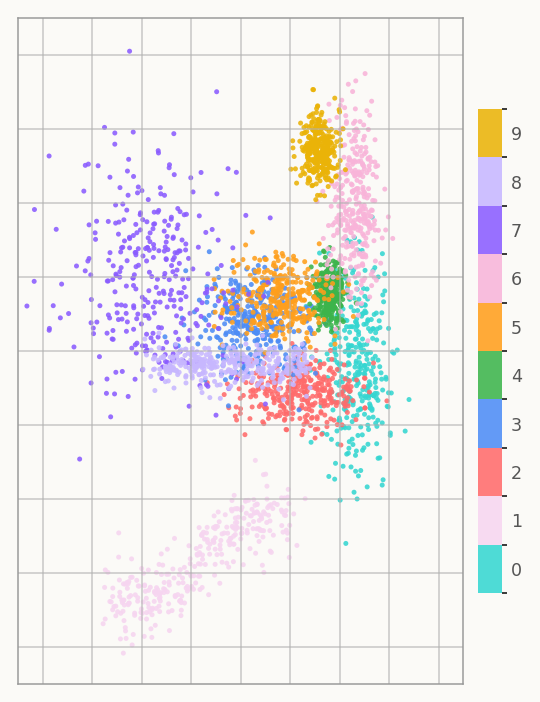
\includegraphics[width=3.8cm]{recon_only_space.png}};

  % explanation box
  \LatentNoteBox{1.00}{2.55}

  \node[
    anchor=west,
    text width=13.15cm,
    align=left,
    font=\footnotesize,
    text=ink
  ] at (1.35,1.82) {
    \textbf{Problem:} With only \textbf{reconstruction loss}, the model may reconstruct data well,
    but the latent space can become \textbf{irregular, discontinuous, and hard to sample from}.
    Random points may fall into weak regions, so generation becomes unreliable.
  };

\end{canvas}
\end{frame}

% ================================================================
% KULLBACK-LEIBLER (KL) DIVERGENCE
% ================================================================

\begin{frame}{Kullback-Leibler (KL) Divergence}

\begin{canvas}

% ================================================================
% OVERLAY 1 — WHAT KL DIVERGENCE MEASURES
% ================================================================

\fill[
    navy!7,
    rounded corners=5pt
]
(1.05,5.75) rectangle (14.95,7.05);

\draw[
    navy,
    line width=1.25pt,
    rounded corners=5pt
]
(1.05,5.75) rectangle (14.95,7.05);

\node[
    anchor=west,
    text width=12.9cm,
    align=left,
    font=\normalsize,
    text=ink
]
at (1.55,6.40)
{
    Measures the divergence between
    $q_{\phi}(z|x)$ and the prior $p(z)$,
    typically $\mathcal{N}(0,I)$.
};


% ================================================================
% OVERLAY 2 — REGULARIZATION PURPOSE
% ================================================================

\only<2->{

    \fill[
        navy!7,
        rounded corners=5pt
    ]
    (1.05,3.25) rectangle (14.95,5.35);

    \draw[
        navy,
        line width=1.25pt,
        rounded corners=5pt
    ]
    (1.05,3.25) rectangle (14.95,5.35);

    \node[
        anchor=west,
        text width=12.9cm,
        align=left,
        font=\normalsize,
        text=ink
    ]
    at (1.55,4.95)
    {
        \textbf{Regularization Purpose}
    };

    \node[
        anchor=west,
        text width=12.9cm,
        align=left,
        font=\normalsize,
        text=ink
    ]
    at (1.55,4.45)
    {
        Promotes a smooth, continuous latent space, fostering:
    };

    \fill[navy]
        (1.95,3.82) circle (2.1pt);

    \node[
        anchor=west,
        font=\normalsize\bfseries,
        text=ink
    ]
    at (2.25,3.95)
    {
        Continuity
    };

    \fill[navy]
        (1.95,3.5) circle (2.1pt);

    \node[
        anchor=west,
        font=\normalsize\bfseries,
        text=ink
    ]
    at (2.25,3.5)
    {
        Completeness
    };
}


% ================================================================
% OVERLAY 3 — KL FORMULA
% ================================================================

\only<3->{

    \fill[
        navy!7,
        rounded corners=5pt
    ]
    (1.05,0.95) rectangle (14.95,2.90);

    \draw[
        navy,
        line width=1.25pt,
        rounded corners=5pt
    ]
    (1.05,0.95) rectangle (14.95,2.90);

    \node[
        anchor=west,
        text width=12.9cm,
        align=left,
        font=\normalsize,
        text=ink
    ]
    at (1.55,2.45)
    {
        \textbf{KL Divergence Formula}
    };

    \node[
        text=navy,
        font=\Large
    ]
    at (8.00,1.65)
    {
        $\displaystyle
        \mathcal{L}_{KL}
        =
        D_{KL}
        \left(
        q_{\phi}(z|x)
        \,\|\, p(z)
        \right)
        =
        \int
        q_{\phi}(z|x)
        \log
        \frac{q_{\phi}(z|x)}
             {p(z)}
        \, dz
        $
    };
}

\end{canvas}

\end{frame}


% ================================================================
% EVIDENCE LOWER BOUND (ELBO)
% ================================================================

\begin{frame}{Evidence Lower Bound (ELBO)}

\begin{canvas}

% ================================================================
% OVERLAY 1 — ELBO OVERVIEW
% ================================================================

\fill[
    navy!7,
    rounded corners=5pt
]
(1.05,4.95) rectangle (14.95,6.65);

\draw[
    navy,
    line width=1.25pt,
    rounded corners=5pt
]
(1.05,4.95) rectangle (14.95,6.65);

\node[
    anchor=west,
    text width=12.9cm,
    align=left,
    font=\normalsize\bfseries,
    text=navy
]
at (1.55,6.28)
{
    ELBO: Overview
};

\node[
    anchor=west,
    text width=12.9cm,
    align=left,
    font=\normalsize,
    text=ink
]
at (1.55,5.65)
{
    ELBO balances two objectives:
    \textbf{Reconstruction Quality}
    and
    \textbf{Latent Space Regularization}.
};


% ================================================================
% OVERLAY 2 — GOAL / LOSS
% ================================================================

\only<2->{

    \fill[
        navy!7,
        rounded corners=5pt
    ]
    (1.05,2.00) rectangle (14.95,4.35);

    \draw[
        navy,
        line width=1.25pt,
        rounded corners=5pt
    ]
    (1.05,2.00) rectangle (14.95,4.35);

    \node[
        anchor=west,
        text width=12.9cm,
        align=left,
        font=\normalsize\bfseries,
        text=navy
    ]
    at (1.55,3.96)
    {
        Goal
    };

    \node[
        anchor=west,
        text width=12.9cm,
        align=left,
        font=\normalsize,
        text=ink
    ]
    at (1.55,3.43)
    {
        Maximizing ELBO is equivalent to minimizing the VAE loss:
    };

    \node[
        text=navy,
        font=\Large
    ]
    at (8.00,2.75)
    {
        $\displaystyle
        \mathcal{L}_{\mathrm{VAE}}
        =
        \mathcal{L}_{\mathrm{recon}}
        +
        \mathcal{L}_{\mathrm{KL}}
        $
    };

    
}

\end{canvas}

\end{frame}
\begin{frame}{ELBO : Impact Visualization}
\begin{canvas}

% =========================================================
% HEADINGS
% =========================================================

\node[
  font=\small\bfseries,
  text=ink,
  align=center
] at (3.15,7.4)
{Only reconstruction loss};

\node[
  font=\small\bfseries,
  text=ink,
  align=center
] at (8.00,7.4)
{Only KL divergence};

\node[
  font=\small\bfseries,
  text=ink,
  align=center
] at (12.85,7.4)
{Reconstruction loss\\and KL divergence};


% =========================================================
% IMAGES
% =========================================================

\node at (3.15,4.75)
{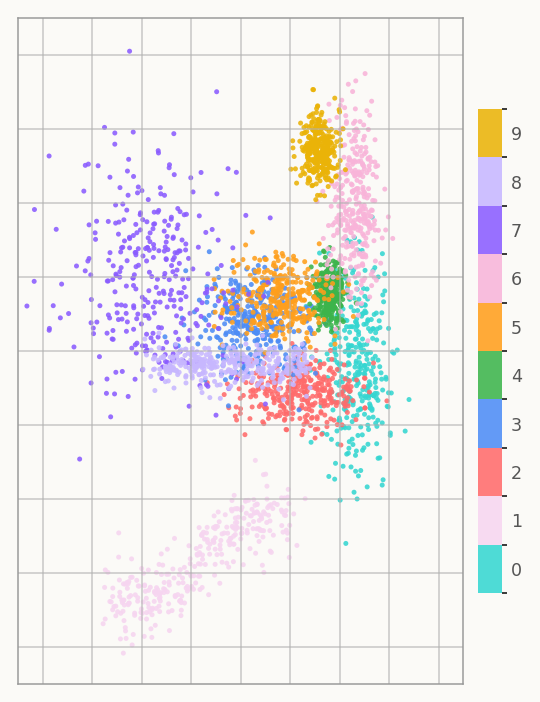
\includegraphics[width=3.2cm]{recon_only_space.png}};

\node at (8.00,4.75)
{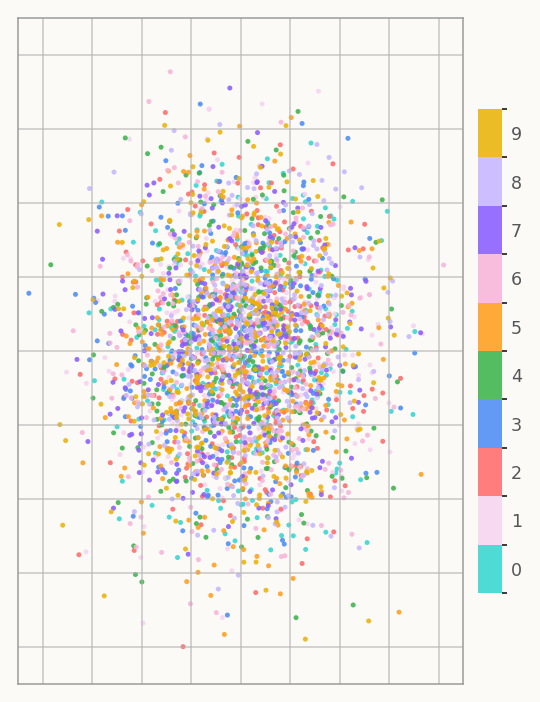
\includegraphics[width=3.2cm]{kl_only_space.png}};

\node at (12.85,4.75)
{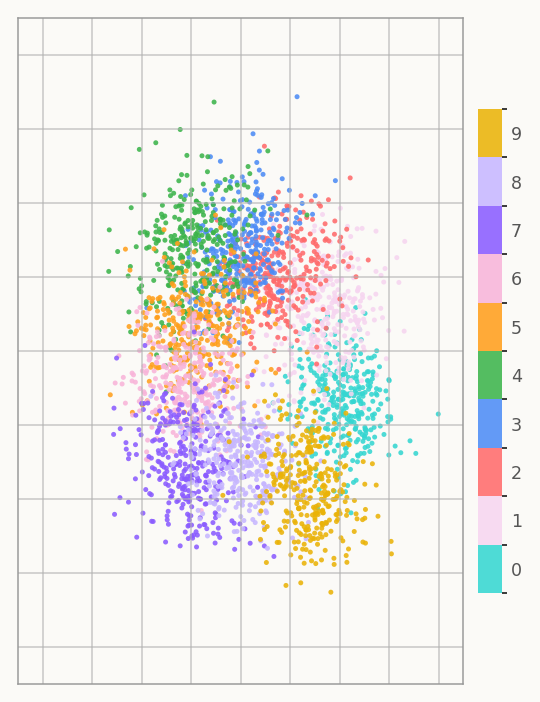
\includegraphics[width=3.2cm]{recon_kl_space.png}};


% =========================================================
% ELBO DIALOG BOX
% =========================================================

\fill[
  navy!7,
  rounded corners=5pt
]
(0.85,0.95) rectangle (15.15,2.45);

\draw[
  navy,
  line width=1.25pt,
  rounded corners=5pt
]
(0.85,0.95) rectangle (15.15,2.45);


\node[
  anchor=west,
  text width=13.3cm,
  align=left,
  font=\footnotesize,
  text=ink
] at (1.25,1.75)
{
  \textbf{ELBO combines both goals:}\quad
  $\displaystyle
  \mathrm{ELBO}
  =
  \mathbb{E}_{q_\phi(z\mid x)}
  \!\left[\log p_\theta(x\mid z)\right]
  -
  D_{KL}\!\left(
  q_\phi(z\mid x)\,\|\,p(z)
  \right)
  $
  \\[5pt]
  In practice:
  \textbf{reconstruct well}
  and
  \textbf{keep the latent space regular}.
};

\end{canvas}
\end{frame}
\endgroup

% #################################################################
%  PART 3  (from part3/part3.tex, unchanged)
%  Wrapped in a group: its colours, styles, macros and templates
%  apply only to its own slides.
% #################################################################
\begingroup
\graphicspath{{assets/part3/frames/}{assets/part3/img/}{assets/part3/walk_frames/}}
% =================================================================
%  VAE presentation — PART 3 (Member 3)
%  What a VAE can do: generation -> latent walk -> CVAE -> applications
%  -> VAEs inside diffusion -> what is next -> closing slide
%  Theme: see ../CLAUDE.md  (preamble copied from ../part2/part2.tex)
%  Images: python gen_images.py  (MNIST digits -> img/, latent-walk
%  animation frames -> walk_frames/, built from 4_to_5_frames/)
%  Build: pdflatex twice.
% =================================================================

\renewcommand{\familydefault}{\rmdefault}

% ---------- Palette ----------
\definecolor{navy}{HTML}{002B55}
\definecolor{steel}{HTML}{4D6FAD}
\definecolor{sky}{HTML}{5DADF5}
\definecolor{teal}{HTML}{3F8C8A}
\definecolor{slate}{HTML}{5B6475}
\definecolor{paper}{HTML}{FBFAF7}
\definecolor{ink}{HTML}{1C2233}
% deeper blue-teal for the "mystery box" = a mix of two palette colours (no new hue)
\colorlet{deepteal}{navy!55!teal}

% ---------- TikZ overlay helpers ----------
\tikzset{
  invisible/.style={opacity=0,text opacity=0},
  visible on/.style={alt={#1{}{invisible}}},
  alt/.code args={<#1>#2#3}{\alt<#1>{\pgfkeysalso{#2}}{\pgfkeysalso{#3}}},
  focus on/.style={alt={#1{draw=teal,line width=1.3pt}{}}},
  emphasis on/.style={alt={#1{draw=deepteal,line width=1.3pt,fill=deepteal!4}{}}},
}

% ---------- Standard diagram styles ----------
\tikzset{
  >={Stealth[length=2mm]},
  arr/.style={->,line width=0.7pt,draw=slate},
  lbl/.style={font=\footnotesize,text=slate,align=center},
  block/.style={trapezium,trapezium stretches=true,minimum width=2.4cm,minimum height=1.55cm,
                line width=0.8pt,font=\bfseries},
  enc/.style={block,shape border rotate=270,fill=steel!12,draw=steel,text=navy},
  dec/.style={block,shape border rotate=90,fill=teal!10,draw=teal,text=teal!70!black},
  param/.style={rectangle,rounded corners=2pt,minimum width=0.95cm,minimum height=0.6cm,
                draw=steel,line width=0.8pt,fill=white,text=navy,font=\normalsize},
  op/.style={circle,draw=slate,line width=0.8pt,fill=white,inner sep=1pt},
  photo/.style={draw=slate!50,line width=0.5pt},
  chip/.style={rectangle,rounded corners=3pt,line width=0.8pt,inner xsep=7pt,inner ysep=4pt,
               font=\footnotesize,fill=white},
  neuron/.style={circle,minimum size=0.48cm,inner sep=0pt,line width=0.7pt,font=\scriptsize},
  mystery/.style={rectangle,rounded corners=5pt,draw=deepteal,line width=1.3pt,fill=white,text=deepteal,
                  font=\fontsize{24}{24}\fontseries{eb}\selectfont},
}

% ---------- Beamer theme ----------
\setbeamercolor{background canvas}{bg=paper}
\setbeamercolor{normal text}{fg=ink}
\setbeamercolor{alerted text}{fg=teal}
\setbeamercolor{structure}{fg=navy}
\setbeamercolor{block title}{bg=navy,fg=white}
\setbeamercolor{block body}{bg=slate!7,fg=ink}
\setbeamertemplate{navigation symbols}{}
\setbeamertemplate{blocks}[rounded][shadow=false]

\newcommand{\stripeTR}[3]{\fill[#3] (#1,9.2) -- ++(#2,0) -- ++(4.5,-3.15) -- ++(-#2,0) -- cycle;}
\newcommand{\stripeBL}[3]{\fill[#3] (#1,-0.2) -- ++(#2,0) -- ++(-4.5,3.15) -- ++(-#2,0) -- cycle;}

\setbeamertemplate{background}{%
  \begin{tikzpicture}[remember picture,overlay,shift={(current page.south west)}]
    \clip (0,0) rectangle (16,9);
  \end{tikzpicture}}

\setbeamertemplate{frametitle}{%
  \begin{tikzpicture}[remember picture,overlay,shift={(current page.north west)}]
    \fill[navy] (0,0) rectangle (16,-1.05);
    \node[anchor=west,text=white,font=\fontseries{eb}\selectfont\Large] at (0.72,-0.525)
      {\insertframetitle};
  \end{tikzpicture}
  \vspace*{0.78cm}}

\setbeamertemplate{footline}{%
  \begin{tikzpicture}[remember picture,overlay,shift={(current page.south west)}]
    \node[anchor=west,font=\scriptsize,text=steel] at (0.72,0.32)
      {Variational Autoencoder \;\textcolor{slate!60}{|}\; CSE200};
    \node[anchor=east,font=\scriptsize\bfseries,text=steel] at (15.3,0.32)
      {\insertframenumber/\inserttotalframenumber};
  \end{tikzpicture}}

% ---------- Page canvas: draw in page coordinates (16 x 9 cm) ----------
% content zone ~ x 0.9..15.1, y 0.9..7.3
\newenvironment{canvas}
  {\begin{tikzpicture}[remember picture,overlay,shift={(current page.south west)}]}
  {\end{tikzpicture}}

% ---------- Reusable drawings ----------
% digit "image" thumbnail:  \thumb[opts]{pos}{digit}
\newcommand{\thumb}[3][]{%
  \node[draw=slate!50,line width=0.5pt,fill=white,minimum size=0.52cm,inner sep=0pt,text=ink,
        font=\small\fontseries{eb}\selectfont,#1] at (#2) {#3};}

% latent-space clusters. #1 = cloud radius (0 = plain points), #2 = scale of cluster centres
\newcommand{\clusters}[2]{%
  \pgfmathsetseed{4242}%
  \foreach \cx/\cy/\sx/\sy/\rot/\col in {
      -2.35/ 1.55/0.34/0.20/ 20/navy,
      -0.25/ 1.85/0.20/0.40/-25/teal,
       2.20/ 1.20/0.40/0.22/ 40/steel,
      -2.05/-1.35/0.30/0.28/  0/slate,
       0.60/-0.45/0.26/0.36/ 60/teal!55!white,
       2.40/-1.65/0.44/0.19/-15/steel!55!white}{%
    \foreach \k in {1,...,22}{%
      \pgfmathsetmacro\rr{min(2.1,sqrt(-2*ln(max(rnd,0.005))))}%
      \pgfmathsetmacro\tt{360*rnd}%
      \pgfmathsetmacro\px{#2*\cx + cos(\rot)*\sx*\rr*cos(\tt) - sin(\rot)*\sy*\rr*sin(\tt)}%
      \pgfmathsetmacro\py{#2*\cy + sin(\rot)*\sx*\rr*cos(\tt) + cos(\rot)*\sy*\rr*sin(\tt)}%
      \ifdim #1pt>0pt \fill[\col,opacity={0.024/#1}] (\px,\py) circle (#1); \fi
      \fill[\col] (\px,\py) circle (0.055);
    }}}
% digit labels next to the clusters (#1 = centre scale)
\newcommand{\clusterlabels}[1]{%
  \foreach \cx/\cy/\dx/\dy/\d in {-2.35/1.55/-0.95/0.25/0, -0.25/1.85/0.55/0.3/1, 2.20/1.20/0.2/0.8/7,
                                  -2.05/-1.35/0.9/-0.5/3, 0.60/-0.45/-0.8/-0.5/5, 2.40/-1.65/-0.15/-0.75/9}
    {\thumb[minimum size=0.42cm,font=\scriptsize\fontseries{eb}\selectfont]{#1*\cx+\dx,#1*\cy+\dy}{\d}}}
% empty latent panel, centred at the current origin (7.4 x 5.9 cm)
\newcommand{\latentpanel}{%
  \fill[white] (-3.7,-2.95) rectangle (3.7,2.95);
  \begin{scope}
    \clip (-3.7,-2.95) rectangle (3.7,2.95);
    \draw[slate!12,line width=0.4pt,step=0.5] (-4,-3) grid (4,3);
    \draw[slate!30,line width=0.5pt] (-3.7,0) -- (3.7,0) (0,-2.95) -- (0,2.95);
  \end{scope}
  \draw[slate!50,line width=0.5pt] (-3.7,-2.95) rectangle (3.7,2.95);
  \node[lbl,anchor=north east] at (3.7,-2.95) {$z_1$};
  \node[lbl,anchor=north east] at (-3.7,2.95) {$z_2$};
  \node[anchor=north west,font=\scriptsize,text=slate] at (-3.62,2.9) {bottleneck (latent) space};}

% number line on [-1,1]:  \numline{pos}{width}
\newcommand{\numline}[2]{%
  \draw[slate!70,line width=0.5pt,<->,>={Stealth[length=1.2mm]}] ($(#1)+(-#2/2-0.18,0)$) -- ($(#1)+(#2/2+0.18,0)$);
  \foreach \v in {-1,0,1}
    \draw[slate!70,line width=0.5pt] ($(#1)+(\v*#2/2,0.05)$) -- ++(0,-0.1)
       node[below=-1.5pt,font=\tiny,text=slate] {$\v$};}
% gaussian on that number line:  \gauss{pos}{width}{mu}{sigma}{height}
\newcommand{\gauss}[5]{%
  \begin{scope}[shift={(#1)}]
    \fill[navy!10] plot[domain={max(-1,#3-3*#4)}:{min(1,#3+3*#4)},samples=45]
          ({\x*#2/2},{#5*exp(-((\x-(#3))^2)/(2*#4*#4))}) -- cycle;
    \draw[navy,line width=0.8pt] plot[domain={max(-1,#3-3*#4)}:{min(1,#3+3*#4)},samples=45]
          ({\x*#2/2},{#5*exp(-((\x-(#3))^2)/(2*#4*#4))});
  \end{scope}}

% face "photo":  \face{pos}{scale}{smile -1..1}{skin}{hair}{style 0 short|1 long|2 curly|3 beard}{bg}{shirt}
\newcommand{\face}[8]{%
  \begin{scope}[shift={(#1)},scale=#2]
    \fill[#7] (-0.6,-0.6) rectangle (0.6,0.6);
    \begin{scope}
      \clip (-0.6,-0.6) rectangle (0.6,0.6);
      \ifcase#6\relax
      \or \fill[#5] (-0.38,-0.62) -- (-0.4,0.06) arc (180:0:0.4) -- (0.38,-0.62) -- cycle;
      \or \foreach \a in {0,30,...,330} \fill[#5] ($(0,0.08)+(\a:0.3)$) circle (0.15);
      \fi
      \fill[#8] (-0.56,-0.62) .. controls (-0.52,-0.42) and (-0.32,-0.36) .. (0,-0.36)
                .. controls (0.32,-0.36) and (0.52,-0.42) .. (0.56,-0.62) -- cycle;
      \fill[#4!85!ink] (-0.09,-0.42) rectangle (0.09,-0.2);
      \fill[#4] (0,0.02) ellipse (0.26 and 0.32);
      \ifnum#6=1\relax\else
        \fill[#5] (-0.27,0.06) .. controls (-0.3,0.44) and (0.3,0.44) .. (0.27,0.06)
                  .. controls (0.18,0.22) and (-0.12,0.26) .. (-0.27,0.06) -- cycle;
      \fi
      \ifnum#6=1\relax
        \fill[#5] (-0.26,0.08) .. controls (-0.22,0.4) and (0.24,0.4) .. (0.26,0.08)
                  .. controls (0.1,0.26) and (-0.1,0.26) .. (-0.26,0.08) -- cycle;
      \fi
      \ifnum#6=3\relax
        \fill[#5] (-0.26,0.0) .. controls (-0.25,-0.42) and (0.25,-0.42) .. (0.26,0.0)
                  -- (0.19,-0.02) .. controls (0.14,-0.2) and (-0.14,-0.2) .. (-0.19,-0.02) -- cycle;
      \fi
      \fill[ink] (-0.1,0.07) circle (0.028) (0.1,0.07) circle (0.028);
      \draw[ink!70,line width=0.5pt] (-0.15,0.15) -- (-0.05,0.16) (0.05,0.16) -- (0.15,0.15);
      \ifnum#6=3\relax\def\mouthcol{white}\else\def\mouthcol{ink}\fi
      \draw[\mouthcol,line width=0.8pt,line cap=round]
            (-0.1,-0.13) .. controls (-0.04,{-0.13-0.11*(#3)}) and (0.04,{-0.13-0.11*(#3)}) .. (0.1,-0.13);
    \end{scope}
    \draw[slate!50,line width=0.5pt] (-0.6,-0.6) rectangle (0.6,0.6);
  \end{scope}}
% the recurring bearded person used on the VAE slides
\newcommand{\person}[2]{\face{#1}{#2}{0.75}{teal!55!white}{slate!55!ink}{3}{steel!10}{steel!60}}

% garbled decoder output (a "meaningless" image)
\newcommand{\garbled}[2]{%
  \begin{scope}[shift={(#1)}]
    \fill[white] (-#2/2,-#2/2) rectangle (#2/2,#2/2);
    \pgfmathsetseed{77}
    \foreach \i in {0,...,7}{\foreach \j in {0,...,7}{%
      \pgfmathsetmacro\g{int(85*rnd*rnd)}%
      \fill[ink!\g] ({-#2/2+\i*#2/8},{-#2/2+\j*#2/8}) rectangle ++(#2/8,#2/8);}}
    \node[text=ink,opacity=0.35,font=\Large\fontseries{eb}\selectfont] at (-0.05,0) {3};
    \node[text=ink,opacity=0.3,rotate=35,font=\Large\fontseries{eb}\selectfont] at (0.08,0.02) {7};
    \draw[slate!50,line width=0.5pt] (-#2/2,-#2/2) rectangle (#2/2,#2/2);
  \end{scope}}

\newcommand{\cmark}{\ding{51}}
\newcommand{\xmark}{\ding{55}}

\title{Variational Autoencoder}
% slides: no hyphenation, ragged text
\hyphenpenalty=10000 \exhyphenpenalty=10000


% ---------- Part-2 extra styles ----------
\tikzset{
  fwd/.style={->,line width=0.8pt,draw=slate},
  grad/.style={->,line width=0.9pt,draw=navy,dash pattern=on 2.6pt off 1.8pt},
  panel/.style={rectangle,rounded corners=4pt,draw=slate!45,line width=0.6pt,fill=white},
  mathbox/.style={rectangle,rounded corners=4pt,draw=navy!45,line width=0.7pt,fill=navy!5,inner sep=6pt},
  keybox/.style={rectangle,rounded corners=4pt,draw=teal,line width=1.0pt,fill=teal!6,inner sep=6pt},
  note/.style={font=\footnotesize,text=ink,align=left},
  badge/.style={circle,text=white,font=\scriptsize\bfseries,inner sep=1.6pt},
}

% ---------- Part-2 reusable drawings ----------
% a "7"-ish pixel image:  \digitg{cell size}{colour}   (origin = lower-left)
\newcommand{\digitg}[2]{%
  \foreach \x/\y in {1/7,2/7,3/7,4/7,5/6,5/5,4/4,3/4,2/3,1/2,1/1,2/1,3/1,4/1,5/1,0/6,2/8,3/8,1/8,5/7}
    \fill[#2] (\x*#1,\y*#1) rectangle ++(#1,#1);
  \draw[slate!50,line width=0.5pt] (0,0) rectangle (7*#1,10*#1);}
% the same image, faded, with a few wrong cells (a reconstruction)
\newcommand{\digitgr}[1]{%
  \foreach \x/\y in {1/7,2/7,3/7,4/7,5/6,5/5,4/4,3/4,2/3,1/2,1/1,2/1,3/1,4/1,5/1,0/6,2/8,3/8,1/8,5/7}
    \fill[ink!60] (\x*#1,\y*#1) rectangle ++(#1,#1);
  \foreach \x/\y in {0/7,4/5,2/2,5/2,3/6}
    \fill[slate!25] (\x*#1,\y*#1) rectangle ++(#1,#1);
  \draw[slate!50,line width=0.5pt] (0,0) rectangle (7*#1,10*#1);}
% mini latent panel centred on the current origin: \mpanel{halfwidth}{halfheight}
\newcommand{\mpanel}[2]{%
  \fill[white] (-#1,-#2) rectangle (#1,#2);
  \begin{scope}
    \clip (-#1,-#2) rectangle (#1,#2);
    \draw[slate!12,line width=0.4pt,step=0.4] (-4,-4) grid (4,4);
    \draw[slate!30,line width=0.5pt] (-#1,0) -- (#1,0) (0,-#2) -- (0,#2);
  \end{scope}
  \draw[slate!50,line width=0.5pt] (-#1,-#2) rectangle (#1,#2);}
% latent scatter: \scat{centre scale}{sigma}{seed}
\newcommand{\scat}[3]{%
  \pgfmathsetseed{#3}%
  \foreach \cx/\cy/\col in {0/1.5/navy, 1.4/0.45/teal, 0.9/-1.25/steel,
                            -0.95/-1.2/slate, -1.4/0.5/teal!55!white}{%
    \foreach \k in {1,...,26}{%
      \pgfmathsetmacro\rr{min(2.2,sqrt(-2*ln(max(rnd,0.005))))}%
      \pgfmathsetmacro\tt{360*rnd}%
      \fill[\col] ({#1*\cx+#2*\rr*cos(\tt)},{#1*\cy+#2*\rr*sin(\tt)}) circle (0.05);}}}
% coloured gaussian: \gaussc{pos}{width}{mu}{sigma}{height}{colour}
\newcommand{\gaussc}[6]{%
  \begin{scope}[shift={(#1)}]
    \fill[#6!12] plot[domain={max(-1,#3-3*#4)}:{min(1,#3+3*#4)},samples=45]
          ({\x*#2/2},{#5*exp(-((\x-(#3))^2)/(2*#4*#4))}) -- cycle;
    \draw[#6,line width=0.8pt] plot[domain={max(-1,#3-3*#4)}:{min(1,#3+3*#4)},samples=45]
          ({\x*#2/2},{#5*exp(-((\x-(#3))^2)/(2*#4*#4))});
  \end{scope}}

% ---------- Part-3 extra styles ----------
\tikzset{
  fade on/.style={alt={#1{opacity=0.22}{}}},
  ychip/.style={rectangle,rounded corners=2pt,draw=slate,line width=0.8pt,fill=white,text=ink,
                minimum width=0.55cm,minimum height=0.5cm,inner sep=2pt,font=\normalsize},
  card/.style={rectangle,rounded corners=4pt,draw=slate!45,line width=0.6pt,fill=white},
  tile/.style={rectangle,rounded corners=2pt,draw=slate!50,line width=0.5pt,fill=white},
  tag/.style={rectangle,rounded corners=2pt,line width=0.6pt,inner xsep=4pt,inner ysep=1.5pt,
              font=\scriptsize,fill=white},
  zdot/.style={circle,fill=navy,draw=white,line width=0.6pt,inner sep=0pt,minimum size=0.2cm},
}

% ---------- Part-3 reusable drawings ----------
% hand-drawn trapezia (exact corners, so arrows can land on the edges)
% \encpoly{cx}{cy}{width}{wide side}{narrow side}  -- wide side on the left
\newcommand{\encpoly}[5]{%
  \filldraw[fill=steel!12,draw=steel,line width=0.8pt,line join=round]
    ({#1-#3/2},{#2-#4/2}) -- ({#1+#3/2},{#2-#5/2}) -- ({#1+#3/2},{#2+#5/2}) -- ({#1-#3/2},{#2+#4/2}) -- cycle;}
% \decpoly{cx}{cy}{width}{wide side}{narrow side}  -- wide side on the right
\newcommand{\decpoly}[5]{%
  \filldraw[fill=teal!10,draw=teal,line width=0.8pt,line join=round]
    ({#1-#3/2},{#2-#5/2}) -- ({#1+#3/2},{#2-#4/2}) -- ({#1+#3/2},{#2+#4/2}) -- ({#1-#3/2},{#2+#5/2}) -- cycle;}
% latent scatter with explicit centres: \blobs{seed}{sigma}{list cx/cy/colour}
\newcommand{\blobs}[3]{%
  \pgfmathsetseed{#1}%
  \foreach \cx/\cy/\col in {#3}{%
    \foreach \k in {1,...,24}{%
      \pgfmathsetmacro\rr{min(2.0,sqrt(-2*ln(max(rnd,0.01))))}%
      \pgfmathsetmacro\tt{360*rnd}%
      \fill[\col] ({\cx+#2*\rr*cos(\tt)},{\cy+#2*\rr*sin(\tt)}) circle (0.045);}}}
% small padlock centred at #1
\newcommand{\padlock}[1]{%
  \begin{scope}[shift={(#1)}]
    \draw[slate,line width=0.9pt] (-0.065,0.02) -- (-0.065,0.09) arc (180:0:0.065) -- (0.065,0.02);
    \fill[slate,rounded corners=0.6pt] (-0.11,-0.12) rectangle (0.11,0.04);
  \end{scope}}
% pixel grid n x n, cell size, colour, lower-left at current origin
\newcommand{\pgrid}[3]{%
  \fill[#3] (0,0) rectangle ({#1*#2},{#1*#2});
  \draw[white,line width=0.35pt,step=#2] (0,0) grid ({#1*#2},{#1*#2});
  \draw[slate!60,line width=0.4pt] (0,0) rectangle ({#1*#2},{#1*#2});}

% MNIST digit in a framed white tile:  \mthumb[opts]{centre}{size in cm}{file}
\newcommand{\mthumb}[4][]{%
  \node[draw=slate!50,line width=0.5pt,fill=white,inner sep=0pt,#1] at (#2) {\includegraphics[width=#3cm]{#4}};}
% 5x5 latent feature map, lower-left at the origin: \lgrid{noise share 0..1}{seed}
% (same seed = same underlying latent, a share of cells replaced by noise)
\newcommand{\lgrid}[2]{%
  \pgfmathsetseed{#2}%
  \foreach \i in {0,...,4}{\foreach \j in {0,...,4}{%
    \pgfmathsetmacro\lgbase{int(14+13*mod(\i*3+\j*2,4))}%
    \pgfmathsetmacro\lgnoise{int(10+65*rnd)}%
    \pgfmathsetmacro\lgpick{rnd}%
    \ifdim\lgpick pt<#1pt \fill[slate!\lgnoise] ({\i*0.14},{\j*0.14}) rectangle ++(0.14,0.14);%
    \else \fill[navy!\lgbase] ({\i*0.14},{\j*0.14}) rectangle ++(0.14,0.14);\fi}}%
  \draw[white,line width=0.3pt,step=0.14] (0,0) grid (0.7,0.7);
  \draw[navy!60,line width=0.5pt] (0,0) rectangle (0.7,0.7);}
% U-Net denoiser block (1.24 x 0.84 cm): \unet{cx}{cy}
\newcommand{\unet}[2]{%
  \begin{scope}[shift={(#1,#2)}]
    \filldraw[fill=navy!6,draw=navy,line width=0.8pt,rounded corners=3pt] (-0.62,-0.42) rectangle (0.62,0.42);
    \foreach \dx/\h in {-0.4/0.56,-0.2/0.4,0/0.24,0.2/0.4,0.4/0.56}
      \fill[navy!45] ({\dx-0.055},-0.3) rectangle ({\dx+0.055},{-0.3+\h});
    \draw[navy!45,line width=0.5pt,dash pattern=on 1.2pt off 1pt] (-0.345,0.2) -- (0.345,0.2) (-0.145,0.04) -- (0.145,0.04);
  \end{scope}}
% idea card (2x2 grid): \idea{left x}{top y}{title}{text}  -- icon tile centre at (x+0.85, top-1.125)
\newcommand{\idea}[4]{%
  \node[card,anchor=north west,minimum width=6.775cm,minimum height=2.25cm] at (#1,#2) {};
  \node[tile,minimum size=1.3cm] at ({#1+0.85},{#2-1.125}) {};
  \node[anchor=north west,font=\small\bfseries,text=navy] at ({#1+1.75},{#2-0.5}) {#3};
  \node[anchor=north west,font=\footnotesize,text=slate,text width=4.75cm,align=left] at ({#1+1.75},{#2-1.0}) {#4};}

% flat icons (Phosphor, MIT licence), converted to TikZ by icons/mk.py
% Phosphor icon "flask-duotone" (MIT licence), 1x1 cm centred on the origin
\newcommand{\icflask}[2]{%
  \fill[#2] (0.3125,-0.3438) -- (-0.3125,-0.3438) .. controls (-0.3238,-0.3438) and (-0.3342,-0.3377) .. (-0.3397,-0.3279) .. controls (-0.3453,-0.3181) and (-0.3451,-0.3061) .. (-0.3393,-0.2964) -- (-0.2202,-0.0980) .. controls (-0.1686,-0.0883) and (-0.0952,-0.0925) .. (-0.0000,-0.1406) .. controls (0.1259,-0.2044) and (0.2138,-0.1911) .. (0.2636,-0.1705) -- (0.3392,-0.2964) .. controls (0.3450,-0.3060) and (0.3451,-0.3180) .. (0.3396,-0.3278) .. controls (0.3341,-0.3376) and (0.3237,-0.3437) .. (0.3125,-0.3438);
  \fill[#1,even odd rule] (0.3660,-0.2804) -- (0.1250,0.1214) -- (0.1250,0.3438) -- (0.1562,0.3438) .. controls (0.1735,0.3438) and (0.1875,0.3577) .. (0.1875,0.3750) .. controls (0.1875,0.3923) and (0.1735,0.4062) .. (0.1562,0.4062) -- (-0.1562,0.4062) .. controls (-0.1735,0.4062) and (-0.1875,0.3923) .. (-0.1875,0.3750) .. controls (-0.1875,0.3577) and (-0.1735,0.3438) .. (-0.1562,0.3438) -- (-0.1250,0.3438) -- (-0.1250,0.1214) -- (-0.3660,-0.2804) .. controls (-0.3775,-0.2996) and (-0.3779,-0.3237) .. (-0.3668,-0.3432) .. controls (-0.3557,-0.3628) and (-0.3350,-0.3750) .. (-0.3125,-0.3750) -- (0.3125,-0.3750) .. controls (0.3350,-0.3750) and (0.3558,-0.3629) .. (0.3669,-0.3433) .. controls (0.3780,-0.3237) and (0.3777,-0.2997) .. (0.3661,-0.2804) -- cycle (-0.0670,0.0967) .. controls (-0.0640,0.1015) and (-0.0625,0.1071) .. (-0.0625,0.1127) -- (-0.0625,0.3438) -- (0.0625,0.3438) -- (0.0625,0.1127) .. controls (0.0625,0.1071) and (0.0640,0.1015) .. (0.0670,0.0967) -- (0.2163,-0.1523) .. controls (0.1694,-0.1616) and (0.1027,-0.1577) .. (0.0141,-0.1129) .. controls (-0.0480,-0.0814) and (-0.1072,-0.0647) .. (-0.1625,-0.0628) -- cycle (-0.3125,-0.3125) -- (-0.2010,-0.1266) .. controls (-0.1454,-0.1199) and (-0.0826,-0.1339) .. (-0.0142,-0.1685) .. controls (0.0600,-0.2061) and (0.1225,-0.2188) .. (0.1733,-0.2188) .. controls (0.1991,-0.2189) and (0.2248,-0.2154) .. (0.2496,-0.2083) -- (0.3125,-0.3125) -- cycle;}
% Phosphor icon "images-duotone" (MIT licence), 1x1 cm centred on the origin
\newcommand{\icimages}[2]{%
  \fill[#2] (0.3750,0.2812) -- (0.3750,-0.0393) -- (0.2823,0.0534) .. controls (0.2701,0.0656) and (0.2504,0.0656) .. (0.2382,0.0534) -- (0.1379,-0.0469) -- (-0.0560,0.1471) .. controls (-0.0619,0.1530) and (-0.0698,0.1563) .. (-0.0781,0.1563) .. controls (-0.0864,0.1563) and (-0.0944,0.1530) .. (-0.1002,0.1471) -- (-0.2500,-0.0027) -- (-0.2500,0.2812) .. controls (-0.2500,0.2985) and (-0.2360,0.3125) .. (-0.2188,0.3125) -- (0.3438,0.3125) .. controls (0.3610,0.3125) and (0.3750,0.2985) .. (0.3750,0.2812);
  \fill[#1,even odd rule] (0.3438,0.3438) -- (-0.2188,0.3438) .. controls (-0.2533,0.3438) and (-0.2812,0.3158) .. (-0.2812,0.2812) -- (-0.2812,0.2188) -- (-0.3438,0.2188) .. controls (-0.3783,0.2188) and (-0.4062,0.1908) .. (-0.4062,0.1562) -- (-0.4062,-0.2812) .. controls (-0.4062,-0.3158) and (-0.3783,-0.3438) .. (-0.3438,-0.3438) -- (0.2188,-0.3438) .. controls (0.2533,-0.3438) and (0.2812,-0.3158) .. (0.2812,-0.2812) -- (0.2812,-0.2188) -- (0.3438,-0.2188) .. controls (0.3783,-0.2188) and (0.4062,-0.1908) .. (0.4062,-0.1562) -- (0.4062,0.2812) .. controls (0.4062,0.3158) and (0.3783,0.3438) .. (0.3438,0.3438) (-0.2188,0.2812) -- (0.3438,0.2812) -- (0.3438,0.0361) -- (0.3044,0.0754) .. controls (0.2927,0.0872) and (0.2768,0.0937) .. (0.2602,0.0937) .. controls (0.2436,0.0937) and (0.2277,0.0872) .. (0.2160,0.0754) -- (0.1379,-0.0027) -- (-0.0340,0.1692) .. controls (-0.0584,0.1936) and (-0.0979,0.1936) .. (-0.1223,0.1692) -- (-0.2188,0.0728) -- cycle (0.2188,-0.2812) -- (-0.3438,-0.2812) -- (-0.3438,0.1562) -- (-0.2812,0.1562) -- (-0.2812,-0.1562) .. controls (-0.2812,-0.1908) and (-0.2533,-0.2188) .. (-0.2188,-0.2188) -- (0.2188,-0.2188) -- cycle (0.3438,-0.1562) -- (-0.2188,-0.1562) -- (-0.2188,-0.0156) -- (-0.0781,0.1250) -- (0.1159,-0.0690) .. controls (0.1281,-0.0812) and (0.1478,-0.0812) .. (0.1600,-0.0690) -- (0.2603,0.0312) -- (0.3438,-0.0523) -- cycle (0.1250,0.1719) .. controls (0.1250,0.1978) and (0.1460,0.2188) .. (0.1719,0.2188) .. controls (0.1978,0.2188) and (0.2188,0.1978) .. (0.2188,0.1719) .. controls (0.2188,0.1460) and (0.1978,0.1250) .. (0.1719,0.1250) .. controls (0.1460,0.1250) and (0.1250,0.1460) .. (0.1250,0.1719);}
% Phosphor icon "magnifying-glass-duotone" (MIT licence), 1x1 cm centred on the origin
\newcommand{\icmagnifyingglass}[2]{%
  \fill[#2] (0.2500,0.0625) .. controls (0.2500,-0.1101) and (0.1101,-0.2500) .. (-0.0625,-0.2500) .. controls (-0.2351,-0.2500) and (-0.3750,-0.1101) .. (-0.3750,0.0625) .. controls (-0.3750,0.2351) and (-0.2351,0.3750) .. (-0.0625,0.3750) .. controls (0.1101,0.3750) and (0.2500,0.2351) .. (0.2500,0.0625);
  \fill[#1,even odd rule] (0.3971,-0.3529) -- (0.2016,-0.1573) .. controls (0.3195,-0.0159) and (0.3054,0.1934) .. (0.1694,0.3177) .. controls (0.0334,0.4419) and (-0.1763,0.4373) .. (-0.3066,0.3071) .. controls (-0.4369,0.1769) and (-0.4418,-0.0328) .. (-0.3176,-0.1689) .. controls (-0.1935,-0.3050) and (0.0158,-0.3194) .. (0.1573,-0.2015) -- (0.3529,-0.3971) .. controls (0.3651,-0.4093) and (0.3849,-0.4093) .. (0.3971,-0.3971) .. controls (0.4093,-0.3849) and (0.4093,-0.3651) .. (0.3971,-0.3529) (-0.3438,0.0625) .. controls (-0.3438,0.2178) and (-0.2178,0.3438) .. (-0.0625,0.3438) .. controls (0.0928,0.3438) and (0.2188,0.2178) .. (0.2188,0.0625) .. controls (0.2188,-0.0928) and (0.0928,-0.2188) .. (-0.0625,-0.2188) .. controls (-0.2178,-0.2186) and (-0.3436,-0.0928) .. (-0.3438,0.0625);}
% Phosphor icon "thumbs-up-duotone" (MIT licence), 1x1 cm centred on the origin
\newcommand{\icthumbsup}[2]{%
  \fill[#2] (-0.1875,0.0938) -- (-0.1875,-0.3125) -- (-0.3750,-0.3125) .. controls (-0.3923,-0.3125) and (-0.4062,-0.2985) .. (-0.4062,-0.2812) -- (-0.4062,0.0625) .. controls (-0.4062,0.0798) and (-0.3923,0.0938) .. (-0.3750,0.0938) -- cycle;
  \fill[#1,even odd rule] (0.4141,0.1870) .. controls (0.3963,0.2072) and (0.3707,0.2188) .. (0.3438,0.2188) -- (0.1250,0.2188) -- (0.1250,0.2812) .. controls (0.1250,0.3675) and (0.0550,0.4375) .. (-0.0312,0.4375) .. controls (-0.0431,0.4375) and (-0.0539,0.4308) .. (-0.0592,0.4202) -- (-0.2068,0.1250) -- (-0.3750,0.1250) .. controls (-0.4095,0.1250) and (-0.4375,0.0970) .. (-0.4375,0.0625) -- (-0.4375,-0.2812) .. controls (-0.4375,-0.3158) and (-0.4095,-0.3438) .. (-0.3750,-0.3438) -- (0.2969,-0.3438) .. controls (0.3441,-0.3438) and (0.3840,-0.3086) .. (0.3899,-0.2617) -- (0.4368,0.1133) .. controls (0.4402,0.1400) and (0.4319,0.1669) .. (0.4141,0.1870) (-0.3750,0.0625) -- (-0.2188,0.0625) -- (-0.2188,-0.2812) -- (-0.3750,-0.2812) -- cycle (0.3748,0.1211) -- (0.3279,-0.2539) .. controls (0.3259,-0.2695) and (0.3126,-0.2813) .. (0.2969,-0.2812) -- (-0.1562,-0.2812) -- (-0.1562,0.0864) -- (-0.0129,0.3732) .. controls (0.0310,0.3644) and (0.0625,0.3259) .. (0.0625,0.2812) -- (0.0625,0.1875) .. controls (0.0625,0.1702) and (0.0765,0.1562) .. (0.0938,0.1562) -- (0.3438,0.1562) .. controls (0.3527,0.1563) and (0.3613,0.1524) .. (0.3672,0.1457) .. controls (0.3731,0.1389) and (0.3759,0.1300) .. (0.3748,0.1211);}


% =================================================================
%  PAGE 2 — generating new data: keep the decoder, sample the prior
% =================================================================
\begin{frame}{Generating New Data}
\begin{canvas}
  \node[anchor=west,font=\footnotesize,text=slate] at (0.95,6.95)
       {Training is over. To make \emph{new} images, we only need half of the network.};
  % ---------- the training pipeline (encoder half fades at step 2) ----------
  \begin{scope}[fade on=<2->]
    \mthumb{1.72,5.35}{1.05}{mnist_7}
    \node[lbl,text=ink] at (1.72,4.55) {$x$};
    \draw[fwd] (2.28,5.35) -- (2.82,5.35);
    \encpoly{3.6}{5.35}{1.35}{2.0}{0.95}
    \node[font=\footnotesize\bfseries,text=navy] at (3.6,5.35) {$q_\phi$};
    \node[lbl,font=\scriptsize] at (3.6,4.12) {encoder};
    \draw[fwd] (4.38,5.35) -- (5.42,5.35);
  \end{scope}
  \node[font=\scriptsize,text=slate,visible on=<2->] at (2.65,3.7) {only needed for \textbf{training}};
  \node[circle,fill=navy!8,draw=navy,line width=0.8pt,text=navy,minimum size=0.84cm] (z) at (5.9,5.35) {$z$};
  \draw[fwd] (z.east) -- (7.46,5.35);
  \decpoly{8.2}{5.35}{1.35}{2.0}{0.95}
  \node[font=\footnotesize\bfseries,text=teal!70!black] at (8.2,5.35) {$p_\theta$};
  \node[lbl,font=\scriptsize] at (8.2,4.12) {decoder};
  \draw[fwd] (8.94,5.35) -- (9.3,5.35);
  % output: reconstruction (1-3) -> a brand-new image (4-)
  \only<1-3>{%
    \mthumb{9.87,5.35}{1.05}{mnist_7_recon}
    \node[lbl,text=ink] at (9.87,4.55) {$\hat{x}$};}
  \only<4->{%
    \mthumb[draw=teal,line width=0.9pt]{9.87,5.35}{1.05}{mnist_3}
    \node[lbl,font=\scriptsize,text=teal!80!black] at (9.87,4.55) {new image};}
  % ---------- step 3: the prior replaces the encoder ----------
  \begin{scope}[visible on=<3->]
    \begin{scope}[shift={(5.9,2.75)}]
      \draw[slate!50,line width=0.5pt] (-1.25,0) -- (1.25,0);
      \fill[navy!10] plot[domain=-1.1:1.1,samples=41] (\x,{1.0*exp(-(\x*\x)/(2*0.36*0.36))}) -- cycle;
      \draw[navy,line width=0.8pt] plot[domain=-1.1:1.1,samples=41] (\x,{1.0*exp(-(\x*\x)/(2*0.36*0.36))});
      \node[zdot] (smp) at (0.38,0.57) {};
    \end{scope}
    \node[anchor=west,font=\scriptsize,text=navy] at (7.3,2.95) {prior $p(z)=\mathcal{N}(0,I)$};
    \draw[fwd,dashed] (smp.north) to[out=90,in=-90] (z.south);
    \node[anchor=east,font=\scriptsize,text=slate] at (5.95,4.3) {sample};
  \end{scope}
  % ---------- right column ----------
  \node[anchor=north west,note,text width=4.0cm,visible on=<1>] at (10.85,6.3)
       {While training, all three stages run: \textcolor{steel}{\textbf{encode}}, \textcolor{navy}{\textbf{sample}},
        \textcolor{teal!80!black}{\textbf{decode}}.};
  \node[anchor=north west,note,text width=4.0cm,visible on=<2-3>] at (10.85,6.3)
       {To generate there is no input image to encode, so take $z$ \textbf{straight from the prior}.};
  \begin{scope}[visible on=<4->]
    \node[anchor=north west,note,text width=4.0cm] at (10.85,6.3)
         {Every new draw gives a \textbf{different} digit:};
    \foreach \k/\d/\yy in {1/3/5.05, 2/8/4.4, 3/6/3.75}{
      \node[anchor=west,font=\scriptsize,text=navy] at (10.95,\yy) {$z^{(\k)}\sim p(z)$};
      \draw[fwd] (12.7,\yy) -- (13.3,\yy);
      \mthumb{13.7,\yy}{0.55}{mnist_\d}}
    \node[anchor=north west,font=\scriptsize,text=slate,text width=4.0cm] at (10.85,3.3)
         {none of them copied from the training set};
  \end{scope}
  % ---------- key box ----------
  \node[keybox,anchor=south west,text width=13.5cm,align=left,font=\footnotesize,visible on=<5->] at (1.1,0.98)
       {The KL term trained every encoding to sit inside $\mathcal{N}(0,I)$, so a random draw lands where the decoder
        already knows what to draw. \textcolor{navy}{\textbf{Learning to generate, not just compress.}}};
\end{canvas}
\end{frame}

% =================================================================
%  PAGE 3 — walking through latent space
% =================================================================
\begin{frame}{Walking Through Latent Space}
\begin{canvas}
  \node[anchor=west,font=\footnotesize,text=slate] at (0.95,6.95)
       {One sample gives one image. What if we don't jump, but \textbf{walk}?};
  % ---------- latent panel ----------
  \begin{scope}[shift={(4.3,4.75)}]
    \mpanel{3.0}{1.8}
    \begin{scope}
      \clip (-3.0,-1.8) rectangle (3.0,1.8);
      \blobs{31}{0.3}{-1.75/-0.75/steel, 1.65/0.75/teal, -1.65/1.05/slate!55, 0.05/1.25/slate!35,
                      2.25/-1.0/steel!45, -0.05/0.05/teal!40}
    \end{scope}
    \node[anchor=north west,font=\scriptsize,text=slate,fill=white,inner sep=1.5pt] at (-2.95,1.75) {latent space};
    \coordinate (A) at (-1.75,-0.75);
    \coordinate (B) at (1.65,0.75);
    \mthumb{-2.5,-1.3}{0.5}{mnist_4}
    \mthumb{2.45,1.3}{0.5}{mnist_5}
    % step 2: the straight line between them
    \begin{scope}[visible on=<2->]
      \draw[navy,line width=0.9pt,dash pattern=on 3pt off 2pt] (A) -- (B);
      \node[font=\scriptsize,text=navy,fill=white,rounded corners=1.5pt,inner sep=1.5pt] at (0.75,-1.35)
           {every point on the line is a valid $z$};
    \end{scope}
    % step 3: four stops along the line
    \begin{scope}[visible on=<3->]
      \foreach \k in {1,2}
        \node[circle,fill=white,draw=navy,line width=0.8pt,inner sep=0pt,minimum size=0.18cm] at ($(A)!{\k/3}!(B)$) {};
      \foreach \k/\t in {0/1,1/2,2/3,3/4}
        \node[badge,fill=navy,font=\tiny\bfseries,inner sep=1.2pt] at ($(A)!{\k/3}!(B)+(-0.14,0.32)$) {\t};
    \end{scope}
    \node[zdot] at (A) {};
    \node[zdot] at (B) {};
    \node[anchor=north,font=\footnotesize,text=navy,fill=white,inner sep=1pt] at ($(A)+(0.12,-0.14)$) {$z_a$};
    \node[anchor=north west,font=\footnotesize,text=navy,fill=white,inner sep=1pt] at ($(B)+(0.08,-0.08)$) {$z_b$};
  \end{scope}
  % ---------- decoder + output box ----------
  \draw[fwd] (7.38,4.75) -- (7.82,4.75);
  \decpoly{8.25}{4.75}{0.8}{1.25}{0.6}
  \node[lbl,font=\scriptsize,text=teal!80!black] at (8.25,3.9) {decoder};
  \draw[fwd] (8.7,4.75) -- (9.08,4.75);
  \node[anchor=south,font=\scriptsize,text=slate] at (10.35,5.98) {decoder output};
  \fill[white] (9.15,3.55) rectangle (11.55,5.95);
  \node at (10.35,4.75) {
\includegraphics[width=2.2cm]{frame_01}};
  \draw[slate!50,line width=0.5pt] (9.15,3.55) rectangle (11.55,5.95);
  % ---------- right column ----------
  \node[anchor=north west,note,text width=3.0cm,visible on=<1-3>] at (11.9,5.95)
       {At $z_a$, the decoder draws a \textbf{4}.};
  \node[anchor=north west,note,text width=3.0cm,visible on=<2-3>] at (11.9,4.7)
       {Now slide $z$ along the line to~$z_b$\,\dots};
  \node[keybox,anchor=north west,text width=2.75cm,align=left,font=\footnotesize,visible on=<4>] at (11.9,6.05)
       {Every step decodes to a \textbf{real-looking} digit.
        \\[4pt] Remember the \textbf{gaps} from Part~1? The KL term filled them.};
  % ---------- filmstrip ----------
  \begin{scope}[visible on=<3->]
    \node[anchor=west,font=\scriptsize,text=slate] at (1.15,1.88) {decoded at each stop:};
    \foreach \k/\f/\xx in {1/01/5.0, 2/04/7.0, 3/07/9.0, 4/10/11.0}{
      \node[tile,minimum size=1.15cm] at (\xx,1.88) {};
      \node at (\xx,1.88) {\includegraphics[width=1.0cm]{frame_\f}};
      \node[badge,fill=navy,font=\tiny\bfseries,inner sep=1.2pt] at (\xx-0.575,2.455) {\k};}
    \foreach \xx in {5.7,7.7,9.7} \draw[fwd] (\xx,1.88) -- ++(0.6,0);
  \end{scope}
\end{canvas}
\end{frame}

% =================================================================
%  PAGE 3b — the walk, animated (frames from gen_images.py)
% =================================================================
\begin{frame}{Walking Through Latent Space}
\begin{canvas}
  \node[inner sep=0pt] at (8.0,4.15) {\animategraphics[autoplay,loop,palindrome,width=14cm]{10}{walk_}{01}{31}};
\end{canvas}
\end{frame}

% =================================================================
%  PAGE 4 — conditional VAE
%  diagram follows the reference: x, y -> encoder -> q(z|x,y) -> z -> decoder <- y
% =================================================================
\begin{frame}{Conditional VAE: Choosing What Comes Out}
\begin{canvas}
  % ---------- step 1: the problem, boxed ----------
  \node[rectangle,rounded corners=4pt,draw=slate!70,line width=0.8pt,fill=slate!6,anchor=south west,
        minimum width=6.8cm,minimum height=1.4cm] at (1.1,5.85) {};
  \node[anchor=north west,font=\footnotesize\bfseries,text=navy] at (1.25,7.17)
       {\textcolor{slate}{\xmark}\; Vanilla VAE: we can't pick the digit};
  \node[circle,fill=navy!8,draw=navy,line width=0.7pt,text=navy,minimum size=0.5cm,inner sep=0pt,font=\footnotesize] (pz) at (1.62,6.3) {$z$};
  \draw[fwd] (pz.east) -- (2.3,6.3);
  \decpoly{2.62}{6.3}{0.6}{0.62}{0.3}
  \draw[fwd] (2.92,6.3) -- (3.3,6.3);
  \foreach \d/\xx in {3b/3.6, 8b/4.1, 1/4.6}
    {\mthumb{\xx,6.3}{0.42}{mnist_\d}}
  \node[font=\footnotesize,text=slate] at (5.12,6.3) {\dots};
  \node[anchor=west,font=\scriptsize,text=slate] at (5.5,6.3) {random digit};
  % ---------- step 2: the fix, boxed ----------
  \begin{scope}[visible on=<2->]
    \node[rectangle,rounded corners=4pt,draw=teal,line width=0.8pt,fill=teal!6,anchor=south west,
          minimum width=6.8cm,minimum height=1.4cm] at (8.1,5.85) {};
    \node[anchor=north west,font=\footnotesize\bfseries,text=teal!80!black] at (8.25,7.17)
         {\cmark\; Conditional VAE (CVAE)};
    \node[anchor=west,font=\footnotesize,text=ink] at (8.3,6.3)
         {give the label $y$ to \textbf{both} halves};
  \end{scope}
  % ---------- step 3: the diagram ----------
  \begin{scope}[visible on=<3->]
    % inputs
    \node[font=\normalsize,text=ink] (x) at (1.55,4.9) {$x$};
    \node[ychip,focus on=<3>] (y1) at (1.55,3.7) {$y$};
    \draw[fwd] (x.east) -- (2.98,4.9);
    \draw[fwd] (y1.east) -- (2.98,3.7);
    % encoder
    \encpoly{3.85}{4.3}{1.6}{2.1}{1.0}
    \node[font=\footnotesize\bfseries,text=navy] at (3.85,4.3) {Encoder};
    \draw[fwd] (4.72,4.3) -- (5.3,4.3);
    % q(z|x,y) as a gaussian, with the sampled point
    \begin{scope}[shift={(6.6,3.7)}]
      \draw[slate!50,line width=0.5pt] (-1.25,0) -- (1.25,0);
      \fill[steel!12] plot[domain=-1.15:1.15,samples=41] (\x,{1.2*exp(-(\x*\x)/(2*0.38*0.38))}) -- cycle;
      \draw[steel,line width=0.8pt] plot[domain=-1.15:1.15,samples=41] (\x,{1.2*exp(-(\x*\x)/(2*0.38*0.38))});
      \draw[steel!70,line width=0.5pt,dash pattern=on 2pt off 1.5pt] (0,0) -- (0,1.2);
      \node[anchor=north,font=\scriptsize,text=steel] at (0,-0.04) {$\bm{\mu}$};
      \node[zdot] (s) at (0.45,0.6) {};
    \end{scope}
    \node[circle,fill=navy!8,draw=navy,line width=0.8pt,text=navy,minimum size=0.76cm] (z) at (8.85,4.5) {$z$};
    \draw[fwd] (s) to[out=65,in=165] (z.west);
    \node[font=\scriptsize,text=steel] at (7.72,5.2) {sampling};
    % decoder, with the label entering from below
    \draw[fwd] (z.east) -- (10.06,4.5);
    \node[ychip,focus on=<3>] (y2) at (9.55,3.25) {$y$};
    \draw[fwd] (y2.north) |- (10.06,4.05);
    \decpoly{10.9}{4.3}{1.6}{2.1}{1.0}
    \node[font=\footnotesize\bfseries,text=teal!70!black] at (10.9,4.3) {Decoder};
    \draw[fwd] (11.76,4.3) -- (12.36,4.3);
    \mthumb{12.95,4.3}{1.05}{mnist_7_m_recon}
    \node[lbl,text=ink] at (12.95,3.5) {$\hat{x}$};
  \end{scope}
  % labels under the blocks
  \node[anchor=north,font=\scriptsize,text=steel,visible on=<3->] at (3.85,2.9) {sees the image \emph{and} its label};
  \node[anchor=north,font=\scriptsize,text=teal!80!black,visible on=<3->] at (10.9,2.9) {draws the digit $y$ asks for};
  % ---------- step 4: the intuition ----------
  \node[mathbox,anchor=south west,text width=5.2cm,minimum height=1.3cm,align=left,font=\footnotesize,visible on=<4->] at (1.1,0.98)
       {The label $y$ says \textbf{\textcolor{teal!80!black}{which}} digit.
        \\[2pt] So $z$ only stores \textbf{\textcolor{navy}{how}} it is written.};
  % ---------- step 5: the payoff ----------
  \begin{scope}[visible on=<5->]
    \node[keybox,anchor=south west,text width=3.3cm,minimum height=1.3cm,align=left,font=\footnotesize] at (8.1,0.98)
         {$y=7$: \textbf{always a 7}, only the \emph{style} varies.};
    \foreach \f/\xx in {7_l/12.35, 7_m/12.9, 7_r/13.45}
      {\mthumb{\xx,1.63}{0.48}{mnist_\f}}
  \end{scope}
\end{canvas}
\end{frame}

% =================================================================
%  PAGE 5 — where VAEs are used (icon grid)
% =================================================================
% \usecase{centre x}{icon centre y}{icon macro}{colour}{title}{one line}
\newcommand{\usecase}[6]{%
  \fill[#4!8] (#1,#2) circle (0.85);
  \begin{scope}[shift={(#1,#2)},scale=1.12] #3{#4}{#4!30} \end{scope}
  \node[font=\normalsize\bfseries,text=#4!80!black] at (#1,{#2-1.2}) {#5};
  \node[font=\footnotesize,text=slate] at (#1,{#2-1.6}) {#6};}

\begin{frame}{Where VAEs Are Used}
\begin{canvas}
  \begin{scope}[visible on=<1->]
    \usecase{4.4}{6.05}{\icmagnifyingglass}{teal}{Anomaly Detection}{bad reconstruction $=$ something unusual}
    \usecase{11.6}{6.05}{\icflask}{navy}{Drug \& Molecule Design}{sample $z$ to get new molecules}
  \end{scope}
  \begin{scope}[visible on=<2->]
    \usecase{4.4}{2.95}{\icthumbsup}{steel}{Recommendation}{a latent ``taste'' for every user}
    \usecase{11.6}{2.95}{\icimages}{teal}{Data Augmentation}{decode extra training examples}
  \end{scope}
\end{canvas}
\end{frame}

% =================================================================
%  PAGE 6 — the VAE inside latent diffusion (Stable Diffusion)
%  columns: 5.64 image/noise, 7.44 encoder/U-Net, 9.09 latent, 10.84 decoder, 12.6 image
% =================================================================
\begin{frame}{How Diffusion Models Use a VAE}
\begin{canvas}
\begin{scope}[shift={(0,-0.25)}]
  % ---------- step 1: the VAE compresses ----------
  \begin{scope}[visible on=<1->]
    \node[anchor=west,font=\footnotesize\bfseries,text=slate] at (1.1,5.6) {1\enspace Compress};
    \person{5.64,5.6}{1.1}
    \node[anchor=north,font=\scriptsize,text=slate] at (5.64,4.85) {$512{\times}512{\times}3$};
    \draw[fwd] (6.34,5.6) -- (6.94,5.6);
    \encpoly{7.44}{5.6}{0.9}{1.2}{0.55}
    \node[anchor=north,font=\scriptsize,text=steel] at (7.44,4.85) {VAE encoder};
    \draw[fwd] (7.89,5.6) -- (8.54,5.6);
    \begin{scope}[shift={(8.59,5.1)},scale=1.4286] \lgrid{0}{11} \end{scope}
    \node[anchor=north,font=\scriptsize,text=navy] at (9.09,4.85) {latent};
    \node[anchor=west,font=\footnotesize,text=ink,align=left] at (9.85,5.6)
         {$64{\times}64{\times}4$\\[1pt]\textbf{\textcolor{navy}{48$\times$ fewer numbers}}};
  \end{scope}
  % ---------- step 2: diffusion works in that small space ----------
  \begin{scope}[visible on=<2->]
    \node[anchor=west,font=\footnotesize\bfseries,text=slate] at (1.1,3.0) {2\enspace Generate};
    \begin{scope}[shift={(5.14,2.5)},scale=1.4286] \lgrid{1}{23} \end{scope}
    \node[anchor=north,font=\scriptsize,text=slate] at (5.64,2.25) {noise};
    \draw[fwd] (6.14,3.0) -- (6.82,3.0);
    \unet{7.44}{3.0}
    \draw[navy,line width=0.7pt,->,>={Stealth[length=1.6mm]}] (7.84,3.42) .. controls (7.84,3.95) and (7.04,3.95) .. (7.04,3.42);
    \node[anchor=west,font=\scriptsize,text=navy] at (7.98,3.78) {$\times 50$};
    \node[chip,draw=slate!70,text=ink,font=\scriptsize,inner ysep=2pt] (prompt) at (7.44,1.55) {``a smiling face''};
    \draw[fwd] (prompt.north) -- (7.44,2.58);
    \draw[fwd] (8.06,3.0) -- (8.59,3.0);
    \begin{scope}[shift={(8.59,2.5)},scale=1.4286] \lgrid{0}{11} \end{scope}
    \node[anchor=north,font=\scriptsize,text=navy] at (9.09,2.25) {latent};
  \end{scope}
  % ---------- step 3: the VAE decoder paints the pixels ----------
  \begin{scope}[visible on=<3->]
    \draw[fwd] (9.59,3.0) -- (10.39,3.0);
    \decpoly{10.84}{3.0}{0.9}{1.2}{0.55}
    \node[anchor=north,font=\scriptsize,text=teal!80!black] at (10.84,2.25) {VAE decoder};
    \draw[fwd] (11.29,3.0) -- (11.94,3.0);
    \person{12.6,3.0}{1.1}
    \node[anchor=north,font=\scriptsize,text=slate] at (12.6,2.25) {new image};
  \end{scope}
\end{scope}
\end{canvas}
\end{frame}

% =================================================================
%  PAGE 7 — what is next for VAEs
% =================================================================
\begin{frame}{What's Next for VAEs}
\begin{canvas}
  % ---------- row 1 ----------
  \begin{scope}[visible on=<1->]
    \idea{1.1}{7.0}{Video generation}{Compressing space \emph{and} time, so AI can make whole clips.}
    \begin{scope}[shift={(1.95,5.875)},scale=1.3]
      \foreach \k/\c in {2/steel!25,1/steel!45,0/white}
        \filldraw[fill=\c,draw=steel,line width=0.6pt] ({-0.3+0.09*\k},{-0.22+0.09*\k}) rectangle ++(0.44,0.32);
      \fill[teal] (-0.13,-0.15) -- (-0.13,0.03) -- (0.02,-0.06) -- cycle;
    \end{scope}
    \idea{8.125}{7.0}{Robots that imagine}{Practising inside a learned latent world before acting.}
    \begin{scope}[shift={(8.975,5.875)},scale=1.3]
      \draw[slate,line width=0.6pt] (-0.15,0.05) -- (-0.15,0.16);
      \fill[teal] (-0.15,0.19) circle (0.035);
      \filldraw[fill=steel!20,draw=navy,line width=0.6pt,rounded corners=2pt] (-0.34,-0.3) rectangle (0.04,0.05);
      \fill[navy] (-0.22,-0.1) circle (0.035) (-0.08,-0.1) circle (0.035);
      \draw[navy,line width=0.5pt] (-0.22,-0.2) -- (-0.08,-0.2);
      \fill[slate!60] (0.1,0.08) circle (0.025) (0.16,0.15) circle (0.033);
      \filldraw[fill=white,draw=slate!70,line width=0.5pt] (0.26,0.27) circle (0.14);
      \fill[teal] (0.2,0.29) circle (0.027);
      \fill[navy] (0.3,0.22) circle (0.027);
      \fill[steel] (0.3,0.33) circle (0.027);
    \end{scope}
  \end{scope}
  % ---------- row 2 ----------
  \begin{scope}[visible on=<2->]
    \idea{1.1}{4.5}{New materials}{Sampling new crystals for better batteries and solar cells.}
    \begin{scope}[shift={(1.95,3.375)},scale=1.3]
      \draw[steel,line width=0.5pt] (-0.27,-0.3) rectangle (0.13,0.1) (-0.13,-0.16) rectangle (0.27,0.24);
      \draw[steel,line width=0.5pt] (-0.27,-0.3) -- (-0.13,-0.16) (0.13,-0.3) -- (0.27,-0.16)
                                    (0.13,0.1) -- (0.27,0.24) (-0.27,0.1) -- (-0.13,0.24);
      \foreach \p in {(-0.27,-0.3),(0.13,-0.3),(0.13,0.1),(-0.27,0.1),(-0.13,-0.16),(0.27,-0.16),(0.27,0.24),(-0.13,0.24)}
        \fill[navy] \p circle (0.045);
      \fill[teal] (0,-0.03) circle (0.07);
    \end{scope}
    \idea{8.125}{4.5}{Reading the brain}{Turning brain scans back into the images a person saw.}
    \begin{scope}[shift={(8.975,3.375)},scale=1.3]
      \foreach \i/\j/\v in {0/0/20,1/0/55,2/0/30,0/1/45,1/1/80,2/1/25,0/2/15,1/2/40,2/2/60}
        \fill[navy!\v] ({-0.4+\i*0.12},{-0.18+\j*0.12}) rectangle ++(0.11,0.11);
      \draw[slate,line width=0.5pt,->,>={Stealth[length=1mm]}] (-0.02,0) -- (0.07,0);
      \person{0.24,0}{0.28}
    \end{scope}
  \end{scope}
  % ---------- closing ----------
  \begin{scope}[visible on=<3->]
    \fill[teal!6,rounded corners=4pt] (1.1,0.98) rectangle (14.9,1.78);
    \draw[teal,line width=1.0pt,rounded corners=4pt] (1.1,0.98) rectangle (14.9,1.78);
    \node[font=\footnotesize,text=ink] at (8.0,1.38)
         {\textbf{\textcolor{steel}{compress}} $\rightarrow$ \textbf{\textcolor{navy}{smooth}} $\rightarrow$
          \textbf{\textcolor{teal!80!black}{sample}}: the same recipe, aimed at new problems.};
  \end{scope}
\end{canvas}
\end{frame}

% =================================================================
%  CLOSING SLIDE — just "Thank you"
% =================================================================
{
\setbeamertemplate{footline}{}
\begin{frame}[plain]
\begin{tikzpicture}[remember picture,overlay,shift={(current page.south west)}]
  \node[text=navy,font=\fontsize{30}{33}\fontseries{eb}\selectfont] at (8,4.5) {Thank You};
\end{tikzpicture}
\end{frame}
}
\endgroup

\end{document}
